%%%%%%%%%%%%%%%%%%%%%%%%%%%%%%%%%%%%%%%%%%%%%%%%%%%%%%%%%%%%%%%%%%%%%%%%%%%%
%% Author template for Operations Research (opre) for articles with e-companion (EC)
%% Mirko Janc, Ph.D., INFORMS, mirko.janc@informs.org
%% ver. 0.96, 11/30/2012
%%%%%%%%%%%%%%%%%%%%%%%%%%%%%%%%%%%%%%%%%%%%%%%%%%%%%%%%%%%%%%%%%%%%%%%%%%%%
%\documentclass[opre,blindrev]{informs3} % current default for manuscript submission
%\documentclass[mnsc,blindrev]{informs3}
%\documentclass{informs3}
\documentclass[informs]{informs3} 


%\usepackage{times}
\OneAndAHalfSpacedXI % current default line spacing
%\OneAndAHalfSpacedXII
%\DoubleSpacedXII
%\DoubleSpacedXI

% If hyperref is used,Latex|DVI->PS|PS->PDF dvi-to-ps driver of choice must be declared as
%   an additional option to the \documentclass. For example
%\documentclass[dvips,opre]{informs3}      % if dvips is used
%\documentclass[dvipsone,opre]{informs3}   % if dvipsone is used, etc.https://www.overleaf.com/project/5c2deea94dfa185b5416465b

%%% OPRE uses endnotes
%%\usepackage{endnotes}
\usepackage{eurosym}
\usepackage{epstopdf}
\usepackage{tabularx}
\usepackage{enumerate}
\usepackage[colorinlistoftodos]{todonotes}
%%\usepackage{mathtools}
%\usepackage{environ}
%\usepackage{pgfplots}
%\usepackage{pgf}
\usepackage{booktabs}
    % define a command which stores all commands that are needed for every
    % `raw gnuplot' call
\newcommand*\GnuplotDefs{
        % set number of samples
        set samples 51;
        %
        % define beta distribution function
        % (copied from <http://gnuplot.sourceforge.net/demo/prob.5.gnu>)
        Binv(p,q)=exp(lgamma(p+q)-lgamma(p)-lgamma(q));
        beta(x,xmin,xmax,p,q)=p<=0||q<=0?1/0:x<xmin||x>xmax?0.0:Binv(p,q)*(x-xmin)**(p-1.0)*(xmax-x)**(q-1.0)/(xmax-xmin)**(q+p-1.0);
}
\DeclareGraphicsExtensions{.eps}
\let\footnote=\endnote
\let\enotesize=\normalsize
\def\notesname{Endnotes}%
\def\makeenmark{\hbox to1.275em{\theenmark.\enskip\hss}}
\def\enoteformat{\rightskip0pt\leftskip0pt\parindent=1.275em
  \leavevmode\llap{\makeenmark}}
  

% Private macros here (check that there is no clash with the style)

% Natbib setup for author-year style
\usepackage{natbib}
 \bibpunct[, ]{(}{)}{,}{a}{}{,}%
 \def\bibfont{\small}%
 \def\bibsep{\smallskipamount}%
 \def\bibhang{24pt}%
 \def\newblock{\ }%
 \def\BIBand{and}%

 \usepackage{multirow}
 \usepackage{multicol}
 \usepackage{subcaption}

%% Setup of theorem styles. Outcomment only one.
%% Preferred default is the first option.
\TheoremsNumberedThrough     % Preferred (Theorem 1, Lemma 1, Theorem 2)
%\TheoremsNumberedByChapter  % (Theorem 1.1, Lema 1.1, Theorem 1.2)
\ECRepeatTheorems

%% Setup of the equation numbering system. Outcomment only one.
%% Preferred default is the first option.
\EquationsNumberedThrough    % Default: (1), (2), ...
%\EquationsNumberedBySection % (1.1), (1.2), ...

% In the reviewing and copyediting stage enter the manuscript number.
\MANUSCRIPTNO{} % When the article is logged in and DOI assigned to it,
                 %   this manuscript number is no longer necessary

%%%%%%%%%%%%%%%%
\begin{document}
%%%%%%%%%%%%%%%%

% Outcomment only when entries are known. Otherwise leave as is and
%   default values will be used.
%\setcounter{page}{1}
%\VOLUME{00}%
%\NO{0}%
%\MONTH{Xxxxx}% (month or a similar seasonal id)
%\YEAR{0000}% e.g., 2005
%\FIRSTPAGE{000}%
%\LASTPAGE{000}%
%\SHORTYEAR{00}% shortened year (two-digit)
%\ISSUE{0000} %
%\LONGFIRSTPAGE{0001} %
%\DOI{10.1287/xxxx.0000.0000}%

% Author's names for the running heads
% Sample depending on the number of authors;
% \RUNAUTHOR{Jones}
% \RUNAUTHOR{Jones and Wilson}
% \RUNAUTHOR{Jones, Miller, and Wilson}
% \RUNAUTHOR{Jones et al.} % for four or more authors
% Enter authors following the given pattern:
%\RUNAUTHOR{Oliveira and Williams-Rioux}

% Title or shortened title suitable for running heads. Sample:
% \RUNTITLE{Bundling Information Goods of Decreasing Value}
% Enter the (shortened) title:
\RUNTITLE{Designing Power Purchasing Agreements}

% Full title. Sample:
% \TITLE{Bundling Information Goods of Decreasing Value}
% Enter the full title:
\TITLE{Designing Power Purchasing Agreements}

% Block of authors and their affiliations starts here:
% NOTE: Authors with same affiliation, if the order of authors allows,
%   should be entered in ONE field, separated by a comma.
%   \EMAIL field can be repeated if more than one author

%\ARTICLEAUTHORS{%
%\AUTHOR{Fernando S. Oliveira}
%\AFF{\EMAIL{bizfmdo@nus.edu.sg}} %, \URL{}}

%Department of Analytics and Operations, National University of Singapore Business School. 

%\AUTHOR{Bertrand Williams-Rioux}
%\AFF{ \EMAIL{xxxxxxxxxxx}}
%Kapsarc, Saudi Arabia 

% Enter all authors
%} % end of the block

\ABSTRACT{%
In this article we address the issue of the design of power purchasing agreements (PPAs). We analyze the complexity of the problem and propose an abstract formulation of the different components and their interactions. We model the bi-level problem representing the interaction between the buyer and the potential sellers studying, analyzing how the optimal weights assigned by the buyer to the different objectives of the PPA influence the generators’ optimal behavior. We apply the model to the analysis of investment in the S.A. energy market.
}
% Sample
%\KEYWORDS{deterministic inventory theory; infinite linear programming duality;
%  existence of optimal policies; semi-Markov decision process; cyclic schedule}

% Fill in data. If unknown, outcomment the field
\KEYWORDS{Electricity; Renewables; Power Purchasing Agreements.}
%\SUBJECTCLASS{Decision analysis: risk-averse players. Games/group decisions: stochastic equilibrium between generators and retailers. Industries: electricity supply chain. }


%\HISTORY{This paper was first submitted on April 12, 1922 and has been with the authors for 83 years for 65 revisions.}

\maketitle
%%%%%%%%%%%%%%%%%%%%%%%%%%%%%%%%%%%%%%%%%%%%%%%%%%%%%%%%%%%%%%%%%%%%%%

% Samples of sectioning (and labeling) in OPRE
% NOTE: (1) \section and \subsection do NOT end with a period
%       (2) \subsubsection and lower need end punctuation
%       (3) capitalization is as shown (title style).
%
%\section{Introduction.}\label{intro} %%1.
%\subsection{Duality and the Classical EOQ Problem.}\label{class-EOQ} %% 1.1.
%\subsection{Outline.}\label{outline1} %% 1.2.
%\subsubsection{Cyclic Schedules for the General Deterministic SMDP.}
%  \label{cyclic-schedules} %% 1.2.1
%\section{Problem Description.}\label{problemdescription} %% 2.

% Text of your paper here

\section{Introduction}\label{Introduction}
An essential feature of the liberalization of the electricity markets has been the use of power purchasing agreements (PPAs) both in the promotion of renewables but also in the transition process from the regulated regime in which the older assets, in many countries, were given long-term contracts that guaranteed the profitability of the productive asset at a pre-agreed rate of return of investment. These contracts are of interest to several countries in the Arab Peninsula, including Saudi Arabia who are pursuing electricity market reform based on the Single Buyer model. Countries representing the Gulf Cooperation Council (GCC) exhibit similar market structures, based on the single buyer model, with consumer tariffs subject to direct subsidies, and indirect subsidies on fuel purchases. In 2004 Oman transitioned from a vertically integrated market, to multiple IPP’s entering into PPAs organized by the Oman Power \& Water Procurement Company (OPWP), \cite{Albadi_2017}. The OPWP will also act as the operator of the wholesale electricity spot market, with plans to begin operation in 2020. 


The Saudi Arabian state owned Saudi Electricity Company (SEC) has announced restructuring plans similar in nature to Oman. The recently formed SEC Principal Buyer Department will play a similar role as OPWP, as the previously vertically integrated company unbundles the ownership of generation assets into new private generation companies. It will be responsible for implementing new PPAs to encourage the growth of private generation companies. The contracts should also conform to the government’s fuel price and tariff reform strategies, and plans to transition to a whole sale spot energy market. 
%Oliveira et al. (2018) provide an overview, and simulate potential impacts, of the restructuring plan. 

The procurement of power from SEC’s current fleet of generating currently operate under long term PPA’s designed to cover the plants investment fixed and non-fuel operating costs. Fuel costs are back by the government, providing SEC with a cashless procurement of fuel from Saudi Aramco, with payables transferred to government account. Despite the favorable cost structure, SEC frequently reports a net loss, which increased from USD 625 million in Q4 2016 to USD 1.47 billion in Q4 2017, \cite{Falcom_2018}. Historically investment decisions have been under the control of the government with electricity tariffs set to regulated government subsidized rates. Under tight market and capital investment controls SEC has reported a return on equity well below global benchmarks, with significant debt to earnings ratio, reported at 6.9 in 2017.

Under the government’s plans to sell SEC’s assets to the private sector, the Principal Buyer will organize new PPA’s similar to contracts currently negotiated with IPP’s that represented 15\% of available capacity in 2017, \cite{ECRA_2018}. However, the current financial position of SEC creates several challenges. One of the first requirement is transitioning fuel procurement to the generators, eliminating government accounting practices for Aramco fuel bills. This includes reform of industrial fuel prices with a gradual transition to a linked reference price,  \cite{Fiscal_Balance_2018}. As a result new PPA’s for the private generation companies will pay significantly more than current fixed rates, for example 1.25 USD/mmbtu charges for natural gas. As variable costs go up tariff levels in the PPA’s must also be adjusted. A challenge for negotiating new contracts will be both protecting consumer welfare while resolving outstanding debt obligations on existing assets.


There are two extreme approaches that we could use to generalize the governments approach to designing PPA’s for transferring assets and their debt obligation. In one case the government approves variable electricity tariffs well above current levels. The tariffs capture targeted fuel price reforms to cover higher operating costs and generate acceptable returns for private generators. %As pointed out in an analysis of the restructuring by Oliveira et al. (2018), 
Reforming fuel and energy prices prior to the unbundling would increase the value of assets sold. This would help to alleviate SEC’s debt obligations and create incentives for generators to prioritize fuel efficiency and possibly diversify into renewable technologies. However this would put strain on government consumer accounts and consumer welfare targets governed by the Electricity and Cogeneration Regulatory Authority.  

Another approach would be to discount the value of the debt obligations transferred through the PPA’s, while preserving the fuel price reform targets and efficiency signals. This would allow the Principal Buyer to set a lower fixed capacity payment in the new PPA’s, and put less strain on consumer accounts budgeted by the government. The government might resist this strategy if it sets greater priority on the SEC to resolve its debt problem. However, this could provide an opportunity for the government to make a strong commit to advancing the restructuring process by creating favorable conditions for private investors in the early stages. This would put less initial pressure on government payments to consumer account, and support a more gradual transition to higher end-user tariffs. We incorporate the two approaches into a case study on the design of new PPA’s in the Saudi market, using the multi-objective optimization approach presented in the following sections.


In theory, the PPA model can support a smooth transition to the wholesale competition model. However, there is clear evidence that when poorly designed PPA’s fail to in this regard, and even become responsible for the failure in the transition process.  For example, Egypt electricity market reform based on IPP investment had to be abandoned after the currency devaluation of 2002-2003 as it doubled the local cost of energy under USD denominated contracts, \cite{Eberhard_2007}. Some states in India had problems due to lack of investment by the IPPs. In South America the markets have equally failed to give the right signals for capacity investment. In the Philippines, on the other hand, the take-or-pay contracts were too generous leading to over investment, as the additional capacity was not required after the Asian financial crises, leading to wasted capacity and very high electricity prices (\citealp{Santiago_Roxas_2010}). 

There are two major models for restructuring the electricity market (e.g., \citealp{Nagayama_2007}): a) wholesale and retail competition, in which there is a partition of the incumbent utilities into generators, retailers, and transport, with the creating of spot markets for electricity and competition among retailers and generators; b) the Single-Buyer model, in which some of the elements of market competition are introduced in the generation and there is a Buyer that is a public company, or owned by the retailers, and buys the energy and capacity required by the market. 

In theory, this Single-Buyer model allows a smoother transition to the wholesale competition model. It tends to be used in developing economies, and it is the preferred model in countries with large oil reserves. Unfortunately, in practice this model has lead to delays in introducing structural reforms until after the liberalization is complete. The Single-Buyer is typically under pressure to pay too much for the electricity and to block further reforms to the market. For these reasons, the Single-Buyer model tends to be expensive for taxpayers and (or) consumers. Taiwan has adopted a single-buyer model (e.g., \citealp{Shih_2007}) in which the IPPs sell to the Taiwan Power Company at the avoidable cost, including both the payments for capacity and energy.


\section{Review of the PPA Literature}\label{Lit_review}

PPAs are long-term performance-based contracts between the electricity generator (seller) and the electricity purchaser (buyer). The buyer may be a representative of the utilities (which we call retailers) and that are responsible for selling the energy to the final consumer, it may be the system operator or the national grid (who then sell the energy purchase to the retailers). These PPAs typically last from 15 to 30 years, depending on the countries and on the generation technology. The contracts provide a risk management instrument that are meant to both protect the investments made by suppliers (generators) of the electricity industry and the consumers that purchase their services. The major functions of the PPAs during the liberalization process were (e.g., \citealp{Kee_2001}): a) to protect consumers and taxpayers from spot market price increases; b) to protect generators from low energy prices, preventing the shut-down of plants due to short-term low prices and, therefore, ensuring the financial viability of the generators during the transition process; c) to reduce any possible market power of generators in the spot market, giving incentives for generation plants to be available at times of high prices, and to coordinate the annual maintenance times. 

There are, usually, several components to a PPA, which may include, e.g., \cite{RCREEE_2012}: a) the energy price which may be fixed, tied to the electricity retail price, tied to the fuel cost; b) a fixed capacity payment; c) the capacity required to be deliverable before the contract starts; d) a minimum delivery obligation which, if not met the generator would be accountable for any losses suffered by the buyer; e) a maximum delivery obligation which stipulates that the buyer may be entitled to pay less for any extra energy generated and the generator may have even to pay for any excess generation. 

Typically, in the initial stages of the liberalization process the renewable generation were given guaranteed feed-in-tariffs that would represent the minimum price received by the generator (which would receive the spot price of the electricity if higher) and would have priority in dispatching. This process was very successful and has lead to a surge of investment in renewable technologies, for example in Portugal and Spain, however this was achieved under state guaranteed prices for all technologies, as feed-in-tariffs were used for renewables and co-generation whereas thermal and large hydro plants kept the old PPAs that were designed to guarantee a rate of return (e.g., \citealp{Amorim_et_al_2013}). These old PPAs, written in the 1990s, had a capacity payment (the largest component) and energy price (to cover the variable costs). The capacity payments are computed annually and cover operational and fixed costs, and are indexed to inflation and exchange rates.


Unfortunately, even when it was a success the PPAs have lead almost always to a large cost for consumers and (or) taxpayers, as it now seems that, given the problems in setting the right level for the feed-in-tariff. \cite{Kashi_2015} has analyzed the IPPs projects in developing countries concluding that they have an incentive to increase the stated investment costs (in order to mitigate risk) and to adopt inefficient power plants as the markups on these plants can be higher.  


For this reason, most electricity markets are now moving to an auction based profit to attribute these PPAs, e.g., \cite{IRENA_2015}. For example, \cite{Shrimali_2016} have analyze the case of India concluding that auctions are cost-effective, saving 58\% from baseline feed-in-tariffs. \cite{Cozzi_2012}, among others, analyzes the case of Brazil’s reverse auctions on wind-power, which were successful in decreasing the PPAs prices and in attracting foreign investment. China has also moved to auctions as a way to determine a market based feed-in-tariff; from 2013, Italy uses auctions to determine how much capacity is installed for each technology under the feed-in-tariffs, avoiding the problems with excess capacity, and awarding the licenses to build to the bidders that offer the largest discount to the pre-defined feed-in-tariff (\citealp{IRENA_2015}). \cite{Newbery_2016} has also concluded that the history of the electricity system in Britain supports the idea that auctions for long-term contracts reduce risk, the cost of capital, nonetheless, these contracts, in order to work, need to include a connection to short-term energy and transmission price signals. 

During these auctions the buyer requests proposals, pre-defining the terms of the PPA, and openly publishing the evaluation criteria used, and the quantity of capacity to be contracted in the auction. It should be noted that competitive bidding has been showed to deliver lower capacity payments (which is the part of the cost of the bid harder to assess) as the generators declare lower capacity costs, when compared to bilateral negotiations between the buyer and the generation companies, \cite{Phadke_2009}. Auctions are, therefore, more cost-effective than feed-in tariffs. Nonetheless, underbidding is the major issue with the auctions because when the price is too low the winner may not deliver the investment. 

For this reason, there has been a recent move from the feed-in-tariffs to closed-bid auction for the PPAs in different technologies. Nonetheless, \cite{Electric_power_2004, delRio_Linares_2014, Shrimali_2016} explain that auctions have a deployment problem (i.e., the winner may not build the contracted plant) and, in order to increase the reliability of the auctioning process, they suggest that: a) competition for the tenders needs to be high, b) access to transmission improved, c) there are credit requirements in the call for projects, d) the tender is better organized using pay-as-bid auctions and e) there should be strong penalties for any delays on delivery.

Brazil is one of the countries that has adopted auction for procurement of energy through long-term contracts between the distribution company and the generators, \cite{Rego_Parente_2013}. The process includes a Dutch-Anglo auction in which, in the first stage, there is a descending clock auction and, in the second stage, there is a single-bid auction. There are two different auctions, one with delivery limit of 3 years (for thermal plants) and another one with delivery of 5 years (for hydro plants). The thermal plants receive a 15 years contract whereas the hydro plants are given a 30 years contract. 

A very similar process is used in the UK. In the inception of the market there was a capacity payment that was a function of the energy price in the electricity pool and of the probability of a supply disruption. In the last 15 years the energy market has moved to a bilateral trading for energy (with a pool for the spot market) with capacity auctions in which the capacity payments are determined. In this capacity market there is a price for the capacity bid into the auction. This capacity auction fixes the capacity payment for 15 years and it takes place 3 years before production is due to start. 

It has been argued that there are several problems with the capacity markets. First, they can be gamed by the generators as it can bid a plant into the spot energy market at a very high price in order to ensure it is not called to generate, and still receive the capacity payment for being available. Second, the market operator has a large control over investment by defining a) the fixed costs used by reference when organizing the auction, b) the deadline to start producing, and c) how many years the auction takes place before delivery.


\section{PPA Design and Selection Using Multi-Objective Optimization} \label{Section_MOO}
In this section we review the literature on the application of multi-objective optimization to the purchasing problem. See, for example, \cite{Ehrgott_2005} and \cite{Taha_2007} for a general introduction to multi-objective optimization. We have chosen to use this tool to compare and evaluate the tenders as it allows the study of problems where there are trade-offs between objectives and it has been used in procurement problems to compare different suppliers and tenders. 

Moreover, the multi-objective decision problem may be, in most cases, solved using linear programming and, therefore, allows the inclusion of realistic details in the representation of the problem and on the decision process faced by the decision-maker. Additionally, it can also be employed in the solution of hierarchical problems in which the buyer has a clear ranking of the different objectives that need to be met. 

The evaluation and selection of the best projects has three main components, e.g.,\cite{KEMA_et_al_2013}: a) pre-assessment; b) economic cost-benefit analysis; c) multi-objective evaluation.

The pre-assessment has three main phases (e.g., \citealp{Asian_Dev_Bank_2010}): a) the eligibility check, in which the projects are analyzed to verify that they meet the call minimum requirements; b) identification of complementarities between the projects and possible issues with project clustering; c) verification that the project data is reliable. 

In practice, for a PPA, some of the minimum requirements may include the identification of the site and demonstration of control over it; proof of security compliance; demonstration of experience in developing at least one commercial electricity generation project; proof that the technology chosen is mature; a demonstration that the project can be connected to the grid; local content requirements both at regional and national levels.


The equivalent tender price model proposed by \cite{Meland_et_al_2011} aims to help in this stage of the selection process by increasing the probability of avoiding project failure due to cost overrun or lack of quality, which is partially achieved by increasing transparency in the tender evaluation process. The main idea of this approach is to identify unreliable projects by comparing the submitted costs with replacement costs obtained using market prices. If the costs submitted and computed by the equivalent tender are very different it is a sign that the tender may not be reliable.


In a second phase we have the economic cost benefit analysis. This assesses the viability of the project given the expected price and cost scenarios, impact on the security of supply and $CO_2$ emissions. If the project is found viable from the perspective of the society (it has a positive net present value), then it proceeds to the ranking stage.


Finally, by using multi-objective optimization the different pre-announced selection criteria are used to rank the projects  (e.g., Asian Development Bank, 2010). The different criteria for evaluation can be classified into classes to which a weight is given. For example (e.g., \citealp{KEMA_et_al_2013}) used the following criteria (weights) pairs: Net present value (0.47), competition enhancement (0.19), system adequacy (0.17), implementation progress (0.11), support of RES (0.06). This list is highly political though, as many other criteria could have been used and even the weights to have been very different. Then, by applying the different multi-objective optimization techniques, which are a small detail given all the policy choices put into the design of the tender process, the projects are selected. 


Other criteria used may include, generically, the price bid, the quality factors, managerial data in terms of accountability and competence, and local content. For example, a very different set of weights and criteria were used by Quebec tender for wind farms (e.g., \citealp{Merrimack_2005}):  a) cost of electricity (0.35), regional content (0.3) national content (0.3), relevant experience (0.1), financial strength (0.05) and project feasibility (0.05). The weights used in the project call for tenders are highly controversial as it puts a very large weight in the local content, which means that instead of trying to benefit electricity consumers the government of Quebec has decided that these consumers should subsidize the production of wind in order to foster their development even if they were not, at the time of the call, competitive internationally. Such a policy has been very successful in China in the development of the wind power equipment industry, e.g., \Citealp{Cozzi_2012}. 

There are three major approaches to solve the multi-objective optimization problem: a) the scalarization technique (e.g., \citealp{Liu_et_al_2000}); b) goal programming; c) multi-level programming. When using the scalarization technique the buyer assumes that all the objectives are of comparable importance and then similar but different weights are assigned to the objectives, which are combined in a single objective scalar function. 

Goal programming is used when all the objectives are of comparable importance and the buyer assigns weights to the objectives and, at the same time, defines the targets that need to be met by each one of them. Then the targets are combined into an objective function composed by the weighted average of the deviation from the targets. The optimal policy is the one that minimizes this function.

On the other hand, multi-level programming is used when there is a hierarchy in the priority level for the objectives. A function representing the weighted average of the highest priority objectives is solved first. Then this solution is used as a constraint in the problem of minimizing the weighted average of the second priority functions. The process then may continue for lower level priority functions by using the solutions of the high priority goals as constraint to the lower priority objectives. This process ensures that the main objectives of the buyer are given a higher possibility of being met, and that deviations from the targets occur for the lower priority objectives.      

Finally, after the tenders are ranked by using the specific method chosen by the buyer, it still needs to select how many of the projects that are of acceptable quality will be selected in the call. 

If there were not enough bids to meet the required capacity then all the qualifying projects are accepted and paid the respective bid prices. This is possibly a very problematic situation as the lack of competition, as discussed earlier, may lead to very high prices: the danger of facing high prices can be prevented by imposing as a qualification criterion a maximum electricity price.

If there are more projects qualified than the required capacity the buyer has to choose the combination of projects to be chosen. This selection can be based on the ranking by the weighted cost, choosing the cheapest; or based on the cost of the higher priority objectives. A second approach is to have a second round of bidding, in which there is an upper bound on the different objectives equal to the bids by the marginal plant project for each one of the targets (as is the case of the Brazilian auctions for the energy price, e.g., \citealp{Rego_Parente_2013}).


\section{Modeling the Generator’s Decision Process } \label{Section_Generator}

Having reviewed the literature on the use of multi-objective optimization for the selection and design of procurement auctions, we are now prepared to start analyzing the decision process used by a generator when biding for a PPA. This analysis is based on the generic hierarchical multi-attribute bid framework proposed \cite{Chua_Li_2000}, which we have adapted for the PPA problem. 

In general the decision problem of the bidder is complex, but can be decomposed into simple interactive parts. The main objective of the bidder is to maximize the expected profit (or net present value) of the project, which needs to take into account a) the probability of winning and b) the return on investment. 


\cite{Chen_1989} proposed a non-linear function to compute the probability of winning as a function of the bid price using a gamma distribution and assuming that the number of competitors follows a Poisson distribution. Nonetheless, this function is not only non-linear but also non-convex, which makes the multi-objective optimization problem much harder to solve. For this reason, \Citealp{Kameshwaran_et_al_2007} approach, based on using piece-wise linear objective functions, seems preferable, as it allows the flexibility of designing a complex bid response function, keeping, at the same time, the linearity of the objective function. Another approach that is based on a log-normal probability of winning, solved as a convex quadratic optimization problem, e.g.,\cite{Capen_et_al_1971}. \cite[Ch. 11]{Phillips_2005} uses a model based on a logistic bid response function to represent the probability of a bid being accepted, taking into account both quality variables, bid price, and the effect of competition. 

Let $x_j$  stand for the level of the selection criteria $j$ out of a list of the $N$ different pre-defined selection criteria defined by the buyer with the weight $\omega_j$  . Let $\pi(x_1, ..., x_j, ..., x_N)$ stand for the profit received by the generator when using the policy $x_1, ..., x_j, ..., x_N$ ; $\rho(x_1, ..., x_j, ..., x_N)$  stands for the probability of winning the bid by using policy $x_1, ..., x_j, ..., x_N$ ; and $\phi(x_1, ..., x_j, ..., x_N)$  be the rating of policy $x_1, ..., x_j, ..., x_N$.       

The objective of the bidder is to maximize the expected profit of the bid as represented by (\ref{eqGenObjective}). The probability of the bid being accepted (\ref{eqGenProbability}) is defined by a logistic bid response function. The bid response function depends on the rating  (\ref{eqGenRating}), in which $\omega_j$  is the weight, pre-announced by the buyer, associated with objective criteria $j$, and it is a weighted average of the different criteria used by the buyer. This rating goes from minus infinity to plus infinity, the higher the better. The logistic probability distribution (\ref{eqGenProbability}) increases to one with a higher rating and it decreases to zero with lower ratings. 


\begin{subequations}\label{eqGeneratorsProblem}
	\begin{align}
	&\mathop {Maximize}\limits_{x_1, ..., x_j, ..., x_N}
	\quad \mathop{\mathbb{E}}(\pi)= \rho(x_1, ..., x_j, ..., x_N)\pi(x_1, ..., x_j, ..., x_N) \label{eqGenObjective}\\
	&\quad \mbox{{\it subject to}:}\notag\\
	&\qquad	\rho(x_1, ..., x_j, ..., x_N)=\frac{1}{1+e^{-\phi(x_1, ..., x_j, ..., x_N)}} \label{eqGenProbability}\\
	&\qquad	\phi(x_1, ..., x_j, ..., x_N) = \sum_{j=1}^{N}\omega_j x_j \label{eqGenRating} 
	\end{align}
\end{subequations}


This internal decision process is based on the inputs that influence the objective function of the bidder and it aims to rationalize the choice of variables to optimally submit to the auction given the different factors considered, such as: a) Competition: do we know who the competitors are and what is there bidding profile? b) The generator’s position in the bidding. c) Risk assessment: analysis of the possible loss incurred by submitting a bid.

The competition depends on the nature of the project, the bidding requirements and economic conditions. Depending on the type of project, degree of technological difficulty, site availability, resource requirements and contractual arrangements, pre-qualification requirements, bidding process, time allocated for preparation of the bids, availability of competitive projects, availability of qualified workers, access to equipment, and regulatory regime, the number of competitors and the keenness of the bidding process changes. 

In our model, the stronger the competition (due to a larger number of competitors) the lower the probability of winning the bid, for the same rating. This means that the minimum rating of the competitors’ increases and, therefore, the probability that, for a given policy, the project is accepted decreases.  


\section{Describing the Components of the Profit Function}\label{Section_profit}

We start by defining the inputs to the generator’s decision process. We have considered three different types of components: a) bid related factors, which depend on the specific project being considered, such as the bidding requirements; b) social and economic conditions; c) firm related factors. 

The profit function considered (\ref{eqProfit}) depends on the specific technology being auctioned, and on possible penalties associated to the call for projects. $p$ is the average energy price; $\delta$ stands for the capacity price; $c$  is the marginal cost;  $f$  are the fixed costs; $l$  is the percentage of local content, $q$ is production and $k$ is capacity. $y$ is the number of years of experience of the management team, and $h$ is an index of the financial strength of the project.


\begin{equation} \label{eqProfit}
\pi(\delta,l,h,y) = (p-c)q+(\delta-f)k
\end{equation}


As local content is a requirement that some governments find necessary to develop industries that are not yet competitive at international prices, it leads to higher industry costs (due to lower productivity from local equipment and local workers). For this reason, we can approximate the relationship between local content and the cost structure of the firms as represented in (\ref{eqMarginalCost}) and (\ref{eqFixedCost}), in which $c_I, f_I$ , stand for the expected marginal and fixed international costs, and $c_L, f_L$  represent the equivalent costs when the plants are built using local content only. 

We also consider the impact of experienced management on costs. Let $\tau$  stand for the impact of number of years of experience on the fixed costs associated to remuneration of the team and $y$ represent the actual number of years of experience. In equation (\ref{eqFixedCost}) the percentage increase in capital with respect to financial strength ($h$) is represented by $\mu$. The financial strength is captured by as the ratio between the bank warranties and the fixed costs of the project. While experienced firms have higher fixed costs, due to hiring better staff, they are also more reliable and, therefore, incur in less risk of the project not meeting the targets.  
%We also include the percentage increase in capital cost based on the years of experience of the management team as the parameter $\xi$.


\begin{equation} \label{eqMarginalCost}
c = c_I(1-l)+c_Ll
\end{equation}

\begin{equation} \label{eqFixedCost}
f = f_I(1-l)+f_Ll+\tau y+\mu h
\end{equation}



The energy supply is represented by (\ref{eqEnergySupply}) and it is a function of the available capacity. The  proportion of capacity available for production, $\theta$, is represented by (\ref{eqTheta}), i.e., the process governing production, which is a function of the local content: the larger the proportion of local content the lower the proportion of capacity available and the faster the deterioration of the plant, $\epsilon_l$. It is also a function of the financial strength of the project, $\epsilon_h$. Another important factor that influences the project feasibility is the risk in project execution, including the risks associated with the project, the generator, the buyer, and the social economic environment. Among the several factors conditioning these risks we would emphasize the degree of subcontracting, the degree of technological challenges, safety hazards, knowledge of the management team, financial strength of the firm, regulatory changes, availability of qualified staff, fuel price fluctuations. The project feasibility needs, therefore, to take into account the risk of execution, which depends on the number of years of experience of the management team $(y)$, on the proportion of local content $(l)$. We would hypothesize that local content leads to higher risk of increased costs whereas years of experience decreases the risk. 

\begin{equation} \label{eqEnergySupply}
q \leq \theta k
\end{equation}

\begin{equation} \label{eqTheta}
\theta = \theta_0-\epsilon_l l +\epsilon_h h
\end{equation}

The energy price is a direct function of the expected production $Q$. This relationship is a demand function, represented by (\ref{eqEnergyDemand}), which would be announced by the buyer in the call for projects. The main idea of including a demand function in the call is to give incentives for the generators to propose larger projects and a lower price. The announcement would also include a minimum expected production that, in effect, also works as a price cap. When the buyer decides to use a feed-in-tariff the $b$ is set to zero and the tariff is equal to $a$.

\begin{equation} \label{eqEnergyDemand}
q = a - bp
\end{equation}

Finally, the buyer can also publish a demand for capacity in the call for projects. The advantage of such a function is that it provides incentives for the generators to reduce the capacity payment in order to develop larger projects. The capacity demand function is represented by (\ref{eqCapacityDemand}): $m$ is the maximum size of the project and $g$ is the decrease in production capacity per monetary unit of increase in its price.


\begin{equation} \label{eqCapacityDemand}
k = m -g \delta
\end{equation}

\section{Analyzing the Interaction Between the Buyer's and the Generator's Decisions }\label{Section_interaction}

In this section we formulate the bilevel problem with the outer level representing the  buyer's perspective, taking into account the factors influencing the bids for PPA's in the inner level, and how they condition the bidder’s behavior. 


\subsection{The Bilevel Problem}\label{Section_problem}

The buyer selects the weights to the different objectives of the call for projects to give the incentives for the optimal bid to meet the buyer’s goals for the tender process. The two level problem is represented by (\ref{eqBuyersProblem}), in which the buyer’s objective (\ref{eqBuyerObjective}) is the weighted gains, for the buyer, arising from the winning bid, when compared to the standardized expected values. In equation (\ref{eqBuyerNormal}) the weights assigned to the bidders decision by the buyer are normalized.

The remaining equations represent the inner level problem of the bidder, where the generators objective (\ref{eqGeneratorObjective})  is to maximize the expected profit of winning the bid. The inner problem is subject to the impact of local content, years of experience and financial strength, on the variable costs, fixed costs, and capacity utilization in equations (\ref{eqBuyerMarginalCost}), (\ref{eqBuyerFixedCost}), and (\ref{eqBuyerTheta}), respectively, as described in Section \ref{Section_profit}. Finally we include the generators capacity limit (\ref{eqBuyerEnergySupply}), the impact of the energy price on the quantity of energy sold (\ref{eqBuyerEnergyDemand}), and the impact of the capacity price on size of the project  (\ref{eqBuyerCapacityDemand}).

Next we include the bid response function (\ref{eqGeneratorProbability}) in the generators decision process, with the rating function defined in (\label{eqBuyerObjective}). We use a standardization process that allows the buyer to rate each bid with the decision variables expressed on the same scale. Each decision criteria is standardized based on a probability distribution, with expected value ${\mathbb{E}()} $ and standard deviation ${\sigma\left(\right)}$. To standardize we take the absolute difference between the decision and its expected value divided by the standard deviation.


\begin{subequations}\label{eqBuyersProblem}
	\begin{align}
	&\mathop {Maximize}\limits_{\omega_{\delta},\omega_{h},\omega_{l},\omega_{p,\omega_{y}}}
	\quad \phi(\delta, h, l, p, y) =  	 \omega_{\delta}\frac{\mathop{\mathbb{E}}\left(\delta\right)-\delta }
	{\sigma\left(l\right)}+\omega_{p}\frac{\mathop{\mathbb{E}}\left(p\right)-p}  {\sigma\left(p\right)} 
	+\omega_{h}\frac{ h-\mathop{\mathbb{E}}\left(h\right)}
	{\sigma\left(h\right)}+\omega_{l}\frac{ l-\mathop{\mathbb{E}}\left(l\right) }{\sigma\left(l\right)}+\omega_{y}\frac{y-\mathop{\mathbb{E}}\left(y\right)}{\sigma\left(y\right)} \label{eqBuyerObjective}\\
	&\quad \mbox{{\it subject to}:}\notag\\
 	&\qquad	 \omega_{\delta}+\omega_{h}+\omega_{l}+\omega_{p}+\omega_{y}=1\label{eqBuyerNormal} \qquad \perp \nu\\
	&\qquad  \omega_{\delta},\omega_{h},\omega_{l},\omega_{p},\omega_{y} \geq 0;\\		
	&\qquad \mathop {Maximize}\limits_{\delta, h, l, p, y}
	\quad \rho(\delta, h, l,p,y)\left(\left(p-c\right)q+\left(\delta-f\right)k\right) \label{eqGeneratorObjective}\\ 
	&\qquad \quad \mbox{{\it subject to}:}\notag\\
	&\qquad \qquad c = c_I(1-l)+c_Ll \label{eqBuyerMarginalCost}\\
	&\qquad \qquad f = f_I(1-l)+f_Ll+\tau y+\mu h \label{eqBuyerFixedCost}\\
	&\qquad \qquad \theta = \theta_0-\epsilon_l l  +\epsilon_h h \label{eqBuyerTheta}\\
    &\qquad \qquad q \leq \theta k	\label{eqBuyerEnergySupply} 	\qquad \perp \zeta_q \geq 0\\
	&\qquad \qquad q = a - bp \label{eqBuyerEnergyDemand}\\	
	&\qquad \qquad k = m -g \delta \label{eqBuyerCapacityDemand}\\
	&\qquad	\qquad \rho(\delta, h, l, p,y)=\frac{1}{1+e^{-\phi(\delta, h, l, p, y)}} \label{eqGeneratorProbability}\\
	&\qquad \qquad  h \leq 1 \label{eqGeneratorFinance}		\qquad \perp \zeta_h \geq 0\\
	&\qquad \qquad  l \leq 1 \label{eqGeneratorLocal}			\qquad \perp \zeta_l \geq 0\\
    &\qquad \qquad  p \geq 0 \label{eqGeneratorPNonN}			\qquad \perp \lambda_p \geq 0\\
    &\qquad \qquad  \delta \geq 0 \label{eqGeneratorDeltaNonN}			\qquad \perp \lambda_{\delta} \geq 0\\
    &\qquad \qquad  l \geq 0 \label{eqGeneratorLocalNonN}			\qquad \perp \lambda_l \geq 0\\
    &\qquad \qquad  h \geq 0 \label{eqGeneratorFinNonN}			\qquad \perp \lambda_h\geq 0\\
    &\qquad \qquad  y\geq 0 \label{eqGeneratorExpNonN}			\qquad \perp \lambda_y \geq 0\\
	\end{align}
\end{subequations}

The $\nu$ stands for the dual variable of the buyer's problem for the weights constraint.  $\zeta_h$ and $\zeta_y$ represent the dual variables of the generator's problem for the number of years of experience and local content, respectively.  $\lambda_p, \lambda_{\delta}, \lambda_l,\lambda_h$ and $\lambda_y$ are the dual on the non-negativity of $p,\delta, l, h$ and $y$, respectively.

The bilevel problem can now be solved as a Mathematical Problem with  Equilbirum Constraints (MPEC), by deriving the optimally conditions of the follower or lower level generators problem, and introducing it into the buyers problem.

Let $\Psi$ represent the generator's Lagrangian.  

$\Psi =\frac{\left(p-c\right)(a - bp )+\left(\delta-f\right)(m -g\delta)}{1+e^{-\phi}} - \zeta_q(a - bp -\theta (m -g\delta))+\left( 1-h\right)\zeta_h+\left( 1-l\right)\zeta_l \\ +\lambda_p p+\lambda_{\delta} \delta+\lambda_l l +\lambda_h h+\lambda_y y  $

Then by taking the partial derivative of the Lagrangian to each one of the generators decision variables and equating them to zero we obtain:

$\frac{\partial \Psi}{\partial \delta} = \frac{m-2\delta g + g f}{1+e^{-\phi}}-\frac{w_{\delta} e^{-\phi} \left(\left(p-c\right)(a - bp )  +\left(\delta-f\right)(m -g\delta)\right)}{\sigma_{\delta}(1+e^{-\phi})^{2}}-g \theta \zeta_q + \lambda_{delta}=0$ ;

$\frac{\partial \Psi}{\partial p} = \frac{a+bc-2bp}{1+e^{-\phi}}-\frac{w_p e^{-\phi} \left(\left(p-c\right)(a - bp )  +\left(\delta-f\right)(m -g\delta)\right)}{\sigma_{p}(1+e^{-\phi})^{2}}+b \zeta_q + \lambda_{p}  =0 $;

$\frac{\partial \Psi}{\partial h} = -\frac{\left(m-g\delta\right)\mu}{1+e^{-\phi}}+{\frac{w_h e^{-\phi} \left(\left(p-c\right)(a - bp )  +\left(\delta-f\right)(m -g\delta)\right)}{\sigma_{h}(1+e^{-\phi})^{2}}}+\zeta_q \epsilon_h \left( m-g\delta\right)-\zeta_h+ \lambda_{h}-\zeta_h  =0 $;

$\frac{\partial \Psi}{\partial l} =  -\frac{\left(m-g\delta\right)f_{L}}{1+e^{-\phi}}+{\frac{w_l e^{-\phi} \left(\left(p-c\right)(a - bp )  +\left(\delta-f\right)(m -g\delta)\right)}{\sigma_{l}(1+e^{-\phi})^{2}}}-\zeta_q \epsilon_l \left( m-g\delta\right)+ \lambda_{l}  -\zeta_l=0 $;

$\frac{\partial \Psi}{\partial y} = -\frac{\left(m-g\delta\right)\tau}{1+e^{-\phi}}+ {\frac{w_y e^{-\phi} \left(\left(p-c\right)(a - bp )  +\left(\delta-f\right)(m -g\delta)\right)}{\sigma_{y}(1+e^{-\phi})^{2}}}+\lambda_{l}  =0 $;

Next we can substitute the non-negativity constraints into the the stationary conditions to get the dual complementary conditions for each primal variable. These are then combined with the equations and constraints from the generators problem to produce the MPEC in terms of the buyers optimization.

\begin{subequations}\label{eqBuyersMPEC}
	\begin{align}
	&\mathop {Maximize}\limits_{\omega_{\delta},\omega_{h},\omega_{l},\omega_{p,\omega_{y}}}
	\quad \phi(\delta, h, l, p, y) =  	 \omega_{\delta}\frac{\mathop{\mathbb{E}}\left(\delta\right)-\delta }
	{\sigma\left(l\right)}+\omega_{p}\frac{\mathop{\mathbb{E}}\left(p\right)-p}  {\sigma\left(p\right)} 
	+\omega_{h}\frac{ h-\mathop{\mathbb{E}}\left(h\right)}
	{\sigma\left(h\right)}+\omega_{l}\frac{ l-\mathop{\mathbb{E}}\left(l\right) }{\sigma\left(l\right)}+\omega_{y}\frac{y-\mathop{\mathbb{E}}\left(y\right)}{\sigma\left(y\right)} \label{eqBuyerObjective}\\
	&\quad \mbox{{\it subject to}:}\notag\\
 	&\qquad	 \omega_{\delta}+\omega_{h}+\omega_{l}+\omega_{p}+\omega_{y}=1\label{eqBuyerNormal} \qquad \perp \nu\\
	&\qquad  \omega_{\delta},\omega_{h},\omega_{l},\omega_{p},\omega_{y} \geq 0;\\
    &\qquad q \leq \theta k	\label{eqBuyerEnergySupply2} 	\qquad \perp \zeta_q\geq 0\\
    &\qquad   h \leq 1 \label{eqGeneratorFinance2}		\qquad \perp \zeta_h\geq 0\\
	&\qquad   l \leq 1 \label{eqGeneratorLocal2}			\qquad \perp \zeta_l\geq 0\\
    & \qquad  \frac{m-2\delta g + g f}{1+e^{-\phi}}-\frac{w_{\delta} e^{-\phi} \left(\left(p-c\right)q +\left(\delta-f\right)k\right)}{\sigma_{\delta}(1+e^{-\phi})^{2}}-g \theta \zeta_q  \geq 0 \qquad\qquad \perp \delta \geq 0\\
    &\qquad \frac{a+bc-2bp}{1+e^{-\phi}}-\frac{w_p e^{-\phi} \left(\left(p-c\right)q+\left(\delta-f\right)k\right)}{\sigma_{p}(1+e^{-\phi})^{2}}+b \zeta_q  \geq 0 \qquad\qquad\qquad \perp p \geq 0\\
    & \qquad -\frac{\left(m-g\delta\right)\mu}{1+e^{-\phi}}+{\frac{w_h e^{-\phi} \left(\left(p-c\right)p +\left(\delta-f\right)k\right)}{\sigma_{h}(1+e^{-\phi})^{2}}}+\zeta_q \epsilon_h k-\zeta_h \geq 0 \qquad \perp h\geq 0\\
    & \qquad -\frac{k f_{L}}{1+e^{-\phi}}+{\frac{w_l e^{-\phi} \left(\left(p-c\right)q  +\left(\delta-f\right)k\right)}{\sigma_{l}(1+e^{-\phi})^{2}}}-\zeta_q \epsilon_l k -\zeta_l \geq 0 \qquad\qquad \perp l\geq 0\\
    &\qquad  -\frac{k\tau}{1+e^{-\phi}}+ {\frac{w_y e^{-\phi} \left(\left(p-c\right)q +\left(\delta-f\right)k\right)}{\sigma_{y}(1+e^{-\phi})^{2}}} \geq 0 \qquad\qquad\qquad\qquad \perp y\geq 0\\  
	&\qquad c = c_I(1-l)+c_Ll \label{eqBuyerMarginalCost2}\\
	&\qquad f = f_I(1-l)+f_Ll+\tau y+\mu h \label{eqBuyerFixedCost2}\\
	&\qquad \theta = \theta_0-\epsilon_l l  +\epsilon_h h \label{eqBuyerTheta2}\\
	&\qquad  q = a - bp \label{eqBuyerEnergyDemand2}\\	
	&\qquad  k = m -g \delta \label{eqBuyerCapacityDemand2}\\
	&\qquad	 \rho(\delta, h, l, p,y)=\frac{1}{1+e^{-\phi(\delta, h, l, p, y)}} \label{eqGeneratorProbability2}\\
	\end{align}
\end{subequations}

    
   
 
   
\subsection{Structural Analysis}\label{Section_analytics}

The bi-level problem (\ref{eqBuyersProblem}) is non-linear and, not convex, due to the functional form of the generator's expected profit (\ref{eqGeneratorObjective}). For this reason, in general, such a problem may have multiple local optima and the Lagrangian of the generator's problem does not have a close-form solution. 

Nonetheless, in this section, we explore some regularities an eventual optimal solution needs to hold, even if the problem is just solved numerically, and we prove that, under some conditions, we are able to compute the optimal solution of this complex problem and establish its uniqueness. 

In  Proposition \ref{prop:prices} we establish a relationship between capacity and energy prices: for any given level of production efficiency, there is a linear relationship between the prices of capacity and energy, so that $l$, $h$, $p$ and $\delta$ are chosen so that production equals available capacity. 

\begin{proposition}\label{prop:prices}
In equilibrium equation (\ref{eqBuyerEnergySupply}) is such that $q = \theta k$  and $p =\frac{a}{b}-\frac{\theta m}{b}+\frac{\theta g }{b}\delta$.
\end{proposition}
%
\proof{Proof:} In equilibrium, from equation (\ref{eqBuyerEnergySupply}), $q = \theta k$ which is equivalent to, based on equations (\ref{eqBuyerEnergyDemand}) and (\ref{eqBuyerCapacityDemand}),  $a - bp = \theta(m -g \delta)$. Then $p =\frac{a -  \theta(m -g \delta)}{b}$ and 
$p =\frac{a}{b}-\frac{\theta m}{b}+\frac{\theta g }{b}\delta$. 
\Halmos
\endproof

In this analysis we assume that all the decision variables are never zero, i.e., the buyer always assigns a positive weight to the different criteria and the generator will always have some experience and some degree of local content. This assumption does not constrain the analysis and allows to concentrate the derivations on the components that matter to the practical solution of the problem.


In Proposition \ref{prop:necessary_buyer} we describe the buyer's necessary conditions of optimality. 
 
 
\begin{proposition}[Buyer's Necessary Conditions]\label{prop:necessary_buyer}
The necessary conditions for optimality of the buyer's problem are as follows:
$\nu - \frac{\delta-\mathop{\mathbb{E}}\left(\delta\right)}{\sigma_{\delta}}=0$;
$\nu - \frac{p-\mathop{\mathbb{E}}\left(p\right)}{\sigma_{p}}=0$;
$\nu + \frac{h-\mathop{\mathbb{E}}\left(h\right)}{\sigma_{h}}=0$;
$\nu + \frac{l-\mathop{\mathbb{E}}\left(l\right)}{\sigma_{l}}=0$;
$\nu + \frac{y-\mathop{\mathbb{E}}\left(y\right)}{\sigma_{y}}=0$;
$\omega_{\delta}+\omega_{h}+\omega_{l}+\omega_{p}+\omega_{y}=1 $;		
$\omega_{\delta},\omega_{h},\omega_{l},\omega_{p},\omega_{y} \geq 0$;
\end{proposition}
%
\proof{Proof:}  
Let $L$ represent the buyer's Lagrangian. Then 
$L =\omega_{\delta}\frac{\mathop{\mathbb{E}}\left(\delta\right)-\delta }
{\sigma\left(l\right)}+\omega_{p}\frac{\mathop{\mathbb{E}}\left(p\right)-p}  {\sigma\left(\delta\right)} 
+\omega_{h}\frac{ h-\mathop{\mathbb{E}}\left(h\right)}
{\sigma\left(h\right)}+\omega_{l}\frac{ l-\mathop{\mathbb{E}}\left(l\right) }{\sigma\left(p\right)}+\omega_{y}\frac{y-\mathop{\mathbb{E}}\left(y\right)}{\sigma\left(y\right)}+\nu (\omega_{\delta}+\omega_{p}+\omega_{h}+\omega_{l}+\omega_{y}-1).$ 
Then by taking the partial derivative of the Lagrangian to each one of the variables and equating them to zero we obtain:
$\frac{\partial L}{\partial \delta} = \nu - \frac{\delta-\mathop{\mathbb{E}}\left(\delta\right)}{\sigma_{\delta}}=0$;
$\frac{\partial L}{\partial p} = \nu - \frac{p-\mathop{\mathbb{E}}\left(p\right)}{\sigma_{p}}=0$;
$\frac{\partial L}{\partial h} = \nu + \frac{h-\mathop{\mathbb{E}}\left(h\right)}{\sigma_{h}}=0$;
$\frac{\partial L}{\partial l} = \nu + \frac{l-\mathop{\mathbb{E}}\left(l\right)}{\sigma_{l}}=0=0$;
$\frac{\partial L}{\partial y} = \nu + \frac{y-\mathop{\mathbb{E}}\left(y\right)}{\sigma_{y}}=0$.
The other conditions are derived directly from the complementarity constraints of the problem. %These are sufficient conditions given that the objective function and constraints are affine.
\Halmos
\endproof 

As a direct corollary of Proposition  \ref{prop:necessary_buyer} it follows that the optimal bid will have the same mark-up (or mark-down) when compared to the expected values. The intriguing component of this result is that this needs to be achieved by the generator without actually observing the targets imposed by the buyer, but only having information about the weights attributed by the buyer to the different components used in the selection of the different projects.  

\begin{corollary}\label{cor:necessary_buyer}
	The percentage gains on each variable when compared to the respective target, are the same:
$\frac{\mathop{\mathbb{E}}\left(\delta\right)-\delta}{\sigma_{\delta}}= \frac{\mathop{\mathbb{E}}\left(p\right)-p}{\sigma_{p}}=\frac{h-\mathop{\mathbb{E}}\left(h\right)}{\sigma_{h}}=\frac{l-\mathop{\mathbb{E}}\left(l\right)}{\sigma_{l}}=
\frac{y-\mathop{\mathbb{E}}\left(y\right)}{\sigma_{y}}$.
\end{corollary}


It follows from Proposition \ref{prop:prices} and Corollary \ref{cor:necessary_buyer} that by determining $\delta$ we obtain $p$ and vice-versa and, therefore, we can derive the close-form relationship between capacity and energy prices as represented in Proposition \ref{prop:price_relation}.


\begin{proposition}\label{prop:price_relation}
	
$\delta=\frac{\left(a-b\mathop{\mathbb{E}}\left(p\right) -\theta m\right)\sigma_{\delta}+b\mathop{\mathbb{E}}\left(\delta\right)\sigma_{p}}{b\sigma_{p}-\theta g\sigma_{\delta}}$;

$p =\frac{-\theta g \mathop{\mathbb{E}}\left(p\right)\sigma_{\delta}+\left(a-\theta m+\theta g \mathop{\mathbb{E}}\left(\delta\right)\right)\sigma_{p}}{b\sigma_{p}-\theta g\sigma_{\delta}}$;	


$\nu =\frac{a-b \mathop{\mathbb{E}}\left(p\right)-\theta m+\theta g \mathop{\mathbb{E}}\left(\delta\right)}{b\sigma_{p}-\theta g\sigma_{\delta}}$.
\end{proposition}

\proof{Proof:}  
From Proposition \ref{prop:prices} we know that $p =\frac{a}{b}-\frac{\theta m}{b}+\frac{\theta g }{b}\delta$, and from  Corollary \ref{cor:necessary_buyer} it is also true that $\frac{\mathop{\mathbb{E}}\left(\delta\right)-\delta}{\sigma_{\delta}}= \frac{\mathop{\mathbb{E}}\left(p\right)-p}{\sigma_{p}}$. Then it follows that $\frac{\mathop{\mathbb{E}}\left(\delta\right)-\delta}{\sigma_{\delta}}=\frac{\mathop{\mathbb{E}}\left(p\right)-(\frac{a}{b}-\frac{\theta m}{b}+\frac{\theta g }{b}\delta)}{\sigma_{p}}$, from which we get 
$\frac{\sigma_{p}}{\sigma_{\delta}}\mathop{\mathbb{E}}\left(\delta\right)-\frac{\sigma_{p}}{\sigma_{\delta}}\delta=\mathop{\mathbb{E}}\left(p\right)-\frac{a}{b}+\frac{\theta m}{b}-\frac{\theta g }{b}\delta$ and equivalently
$\delta=\frac{\frac{\sigma_{p}}{\sigma_{\delta}}\mathop{\mathbb{E}}\left(\delta\right)-\mathop{\mathbb{E}}\left(p\right)+\frac{a}{b}-\frac{\theta m}{b}}{\frac{\sigma_{p}}{\sigma_{\delta}}-\frac{\theta g }{b}}$. Then we multiply the numerator and the denominator by $b\sigma_{\delta}$ and obtain:
$\delta=\frac{\left(a-b\mathop{\mathbb{E}}\left(p\right) -\theta m\right)\sigma_{\delta}+b\mathop{\mathbb{E}}\left(\delta\right)\sigma_{p}}{b\sigma_{p}-\theta g\sigma_{\delta}}$.

Moreover, as $p =\frac{a}{b}-\frac{\theta m}{b}+\frac{\theta g }{b}\delta$ it then follows that $p =\frac{a}{b}-\frac{\theta m}{b}+\frac{\theta g }{b}\left(   \frac{\left(a-b\mathop{\mathbb{E}}\left(p\right) -\theta m\right)\sigma_{\delta}+b\mathop{\mathbb{E}}\left(\delta\right)\sigma_{p}}{b\sigma_{p}-\theta g\sigma_{\delta}}  \right) $, which is equivalent to
$p =\frac{\frac{a}{b}\left(b\sigma_{p}-\theta g\sigma_{\delta}\right)-\frac{\theta m}{b}\left(b\sigma_{p}-\theta g\sigma_{\delta}\right)+\frac{\theta g }{b}\left(   \left(a-b\mathop{\mathbb{E}}\left(p\right) -\theta m\right)\sigma_{\delta}+b\mathop{\mathbb{E}}\left(\delta\right)\sigma_{p}\right)}{b\sigma_{p}-\theta g\sigma_{\delta}}$ and simplified to
$p =\frac{-\theta g \mathop{\mathbb{E}}\left(p\right)\sigma_{\delta}+\left(a-\theta m+\theta g \mathop{\mathbb{E}}\left(\delta\right)\right)\sigma_{p}}{b\sigma_{p}-\theta g\sigma_{\delta}}$.

Finally, as from Proposition \ref{prop:necessary_buyer},
$\nu - \frac{p-\mathop{\mathbb{E}}\left(p\right)}{\sigma_{p}}=0$. It then follows that

$\nu = \frac{\left(\frac{-\theta g \mathop{\mathbb{E}}\left(p\right)\sigma_{\delta}+\left(a-\theta m+\theta g \mathop{\mathbb{E}}\left(\delta\right)\right)\sigma_{p}}{b\sigma_{p}-\theta g\sigma_{\delta}} \right)-\mathop{\mathbb{E}}\left(p\right)}{\sigma_{p}}$, which simplifies to:
$\nu =\frac{a-b \mathop{\mathbb{E}}\left(p\right)-\theta m+\theta g \mathop{\mathbb{E}}\left(\delta\right)}{b\sigma_{p}-\theta g\sigma_{\delta}}$.
\Halmos
\endproof 

By the analysis of Corollary \ref{cor:necessary_buyer} it is evident that from the perspective of the buyer the weights to be assigned to the different components of the rating function are undetermined. 

Moreover, given that we were able to compute the optimal prices in Proposition  \ref{prop:price_relation}, we can now determine the optimal value of the objective function of the buyer as well as of the probability of the optimal bid being accepted, as proved in Proposition \ref{prop:optimal_bid}.



\begin{proposition}\label{prop:optimal_bid}
The optimal rating is $\phi=-\nu =-\frac{a-b \mathop{\mathbb{E}}\left(p\right)-\theta m+\theta g \mathop{\mathbb{E}}\left(\delta\right)}{b\sigma_{p}-\theta g\sigma_{\delta}}$ and that probability of the optimal bid is accepted equals $\rho=\frac{1}{1+e^{\nu}}=\frac{1}{1+e^{\frac{a-b \mathop{\mathbb{E}}\left(p\right)-\theta m+\theta g \mathop{\mathbb{E}}\left(\delta\right)}{b\sigma_{p}-\theta g\sigma_{\delta}}  }}$.

\end{proposition}
%
\proof{Proof:} 
From Proposition \ref{prop:necessary_buyer} we know that in the optimal solution all the ratios $\frac{\mathop{\mathbb{E}}\left(x\right)-x}{\sigma_{x}} = \nu$ for all $x = {h, l, y}$, and $\frac{\mathop{x-\mathbb{E}}\left(x\right)}{\sigma_{x}} = \nu$ for all $x = {\delta, p}$. Additionally, we know from Proposition \ref{prop:price_relation} that the optimal $\nu =\frac{a-b \mathop{\mathbb{E}}\left(p\right)-\theta m+\theta g \mathop{\mathbb{E}}\left(\delta\right)}{b\sigma_{p}-\theta g\sigma_{\delta}}$ and from the necessary conditions of optimality 
$\omega_{\delta}+\omega_{h}+\omega_{l}+\omega_{p}+\omega_{y}=1 $ and 		
$\omega_{\delta},\omega_{h},\omega_{l},\omega_{p},\omega_{y} \geq 0$. 

Then, by replacing $\nu$ into the objective function (\ref{eqBuyerObjective}), 
$\phi=\omega_{\delta}\frac{\mathop{\mathbb{E}}\left(\delta\right)-\delta }
{\sigma\left(l\right)}+\omega_{p}\frac{\mathop{\mathbb{E}}\left(p\right)-p}  {\sigma\left(\delta\right)} 
+\omega_{h}\frac{ h-\mathop{\mathbb{E}}\left(h\right)}
{\sigma\left(h\right)}+\omega_{l}\frac{ l-\mathop{\mathbb{E}}\left(l\right) }{\sigma\left(p\right)}+\omega_{y}\frac{y-\mathop{\mathbb{E}}\left(y\right)}{\sigma\left(y\right)}$, we obtain:
$\phi=-\omega_{\delta}\nu-\omega_{p}\nu 
-\omega_{h}\nu-\omega_{l}\nu-\omega_{y}\nu = \phi=-\nu$. Therefore, 
$\phi=-\nu =-\frac{a-b \mathop{\mathbb{E}}\left(p\right)-\theta m+\theta g \mathop{\mathbb{E}}\left(\delta\right)}{b\sigma_{p}-\theta g\sigma_{\delta}}$.  Then, from equation (\ref{eqGeneratorProbability}) it follows that the probability that the optimal bid is accepted is equal to  
$\rho=\frac{1}{1+e^{\nu}}=\frac{1}{1+e^{\frac{a-b \mathop{\mathbb{E}}\left(p\right)-\theta m+\theta g \mathop{\mathbb{E}}\left(\delta\right)}{b\sigma_{p}-\theta g\sigma_{\delta}}  }}$.\Halmos
\endproof


Interestingly enough, it also follows from Corollary \ref{cor:necessary_buyer} and Proposition \ref{prop:price_relation} that the optimal bids for the financial strength $h$, years of experience $y$ and local content $l$ can be all obtained by solving the buyer's problem, as proved in Proposition \ref{prop:optimal_l_h_y}.



\begin{proposition}\label{prop:optimal_l_h_y}

	
	The optimal financial strength equals: 	
	$h =\mathop{\mathbb{E}}\left(h\right)-  \sigma_{h} \frac{a-b \mathop{\mathbb{E}}\left(p\right)-\theta m+\theta g \mathop{\mathbb{E}}\left(\delta\right)}{b\sigma_{p}-\theta g\sigma_{\delta}}$;
	
	The optimal local content equals: 	
	$l =\mathop{\mathbb{E}}\left(l\right)-  \sigma_{l} \frac{a-b \mathop{\mathbb{E}}\left(p\right)-\theta m+\theta g \mathop{\mathbb{E}}\left(\delta\right)}{b\sigma_{p}-\theta g\sigma_{\delta}}$;

	The optimal number of years of experience equals:	
	$y =\mathop{\mathbb{E}}\left(y\right)-  \sigma_{y} \frac{a-b \mathop{\mathbb{E}}\left(p\right)-\theta m+\theta g \mathop{\mathbb{E}}\left(\delta\right)}{b\sigma_{p}-\theta g\sigma_{\delta}}$.
	
	
\end{proposition}
%
\proof{Proof:}
From Proposition \ref{prop:necessary_buyer}, we know that for x = \{h, l, y\},  $\frac{\mathop{\mathbb{E}}\left(x\right)-x}{\sigma_{x}} = \nu$,  which is equivalent to $x =\mathop{\mathbb{E}}\left(x\right)- \nu \sigma_{x}$. We know from Proposition \ref{prop:price_relation} that $\nu =\frac{a-b \mathop{\mathbb{E}}\left(p\right)-\theta m+\theta g \mathop{\mathbb{E}}\left(\delta\right)}{b\sigma_{p}-\theta g\sigma_{\delta}}$. It the follows that:


$h =\mathop{\mathbb{E}}\left(h\right)-  \sigma_{h} \frac{a-b \mathop{\mathbb{E}}\left(p\right)-\theta m+\theta g \mathop{\mathbb{E}}\left(\delta\right)}{b\sigma_{p}-\theta g\sigma_{\delta}}$;


$l =\mathop{\mathbb{E}}\left(l\right)-  \sigma_{l} \frac{a-b \mathop{\mathbb{E}}\left(p\right)-\theta m+\theta g \mathop{\mathbb{E}}\left(\delta\right)}{b\sigma_{p}-\theta g\sigma_{\delta}}$;

$y =\mathop{\mathbb{E}}\left(y\right)-  \sigma_{y} \frac{a-b \mathop{\mathbb{E}}\left(p\right)-\theta m+\theta g \mathop{\mathbb{E}}\left(\delta\right)}{b\sigma_{p}-\theta g\sigma_{\delta}}$.


.\Halmos
\endproof




\subsection{Simple Problem with Capacity and Energy Prices as Variables}

Given the complexity of the problem, it is not possible to derive the close-form solution of the necessary conditions for local optimality.  For this reason, in order to better understand the nature of the problem, and to build a framework with which to assess the performance of the numerical solutions, in this subsection we propose the analysis of an instance of the general problem analyzed so far. We consider that the only decision variables of the generator considered in the auction are the capacity and energy prices. Under this condition, the new bilevel problem is represented by equations \ref{eqBuyersSimple}, in which $c$, $f$, and $\theta$ are given parameters.

\begin{subequations}\label{eqBuyersSimple}
	\begin{align}
	&\mathop {Maximize}\limits_{\omega_{\delta},\omega_{p}}
	\quad \phi(\delta, p) =  	 \omega_{\delta}\frac{\mathop{\mathbb{E}}\left(\delta\right)-\delta }
	{\sigma\left(l\right)}+\omega_{p}\frac{\mathop{\mathbb{E}}\left(p\right)-p}  {\sigma\left(p\right)}  \label{eqBuyerObjectiveSimple}\\
	&\quad \mbox{{\it subject to}:}\notag\\
	&\qquad	 \omega_{\delta}+\omega_{p}=1\label{eqBuyerNormalSimple} \qquad \perp \nu\\
	&\qquad  \omega_{\delta},\omega_{p}, \geq 0;\\		
	&\qquad \mathop {Maximize}\limits_{\delta, p}
	\quad \rho(\delta,p)\left(\left(p-c\right)q+\left(\delta-f\right)k\right) \label{eqGeneratorObjectiveSimple}\\ 
	&\qquad \quad \mbox{{\it subject to}:}\notag\\
	&\qquad \qquad q \leq \theta k	\label{eqBuyerEnergySupplySimple} 	\qquad \perp \zeta_q\\
	&\qquad \qquad q = a - bp \label{eqBuyerEnergyDemandSimple}\\	
	&\qquad \qquad k = m -g \delta \label{eqBuyerCapacityDemandSimple}\\
	&\qquad	\qquad \rho(\delta, p)=\frac{1}{1+e^{-\phi(\delta, p)}} \label{eqGeneratorProbabilitySimple}\\
	&\qquad \qquad  \delta, p, \zeta_q\geq 0 \label{eqGeneratorNon-NegativeSimple}
	\end{align}
\end{subequations}

The buyer's problem is very similar to the previous one and all the conclusions of our analysis so far still hold for the bilinear program \ref{eqBuyersSimple}. In Proposition \ref{prop:necessary_generator} we summarize the generator's necessary conditions for optimality; these are not sufficient as the problem is not convex.



\begin{proposition}[Generator's Necessary Conditions]\label{prop:necessary_generator}
	The necessary conditions for optimality of the generator's problem are as follows:
	
$\frac{m-2\delta g + g f}{1+e^{-\phi}}-\frac{w_{\delta} e^{-\phi} \left(\left(p-c\right)(a - bp )  +\left(\delta-f\right)(m -g\delta)\right)}{\sigma_{\delta}(1+e^{-\phi})^{2}}-g \theta \zeta_q =0$;


$\frac{a+bc-2bp}{1+e^{-\phi}}-\frac{w_p e^{-\phi} \left(\left(p-c\right)(a - bp )  +\left(\delta-f\right)(m -g\delta)\right)}{\sigma_{p}(1+e^{-\phi})^{2}}+b \zeta_q =0$;

$(a - bp -\theta (m -g\delta)) = 0 \perp \zeta_q$; 

$\delta, p, \zeta_q \geq 0$.
\end{proposition}
%
\proof{Proof:}  
Let $\Psi$ represent the generator's Lagrangian. Then 
%$\Psi =\frac{\left(p-c\right)(a - bp )+\left(\delta-f\right)(m -g\delta)}{1+e^{-\omega_{\delta}\frac{\mathop{\mathbb{E}}\left(\delta\right)-\delta }
%		{\sigma\left(l\right)}-\omega_{p}\frac{\mathop{\mathbb{E}}\left(p\right)-p}  {\sigma\left(p\right)}}   } - \zeta_q(a - bp -\theta (m -g\delta))$. 
$\Psi =\frac{\left(p-c\right)(a - bp )+\left(\delta-f\right)(m -g\delta)}{1+e^{-\phi}} - \zeta_q(a - bp -\theta (m -g\delta))$. 



Then by taking the partial derivative of the Lagrangian to each one of the prices and equating them to zero we obtain:

$\frac{\partial \Psi}{\partial \delta} = \frac{m-2\delta g + g f}{1+e^{-\phi}}-\frac{w_{\delta} e^{-\phi} \left(\left(p-c\right)(a - bp )  +\left(\delta-f\right)(m -g\delta)\right)}{\sigma_{\delta}(1+e^{-\phi})^{2}}-g \theta \zeta_q =0$;



$\frac{\partial \Psi}{\partial p} = \frac{a+bc-2bp}{1+e^{-\phi}}-\frac{w_p e^{-\phi} \left(\left(p-c\right)(a - bp )  +\left(\delta-f\right)(m -g\delta)\right)}{\sigma_{p}(1+e^{-\phi})^{2}}+b \zeta_q =0$;

The other conditions are derived directly from the complementarity constraints of the problem: 
$(a - bp -\theta (m -g\delta)) = 0 \perp \zeta_q$; and $\delta, p, \zeta_q \geq 0$.
\Halmos
\endproof 


It is clear from Proposition \ref{prop:necessary_generator} that the generator's problem, by itself is not amenable to a close-form solution. Instead, we need to solve a system of equations incorporating both the necessary conditions of optimality for both the buyer and the generator. Proposition \ref{prop:solution_simple} summarizes the optimal solution of the problem. 

\begin{proposition}[Optimal Solution]\label{prop:solution_simple}


$\delta = \frac{\left(a - b\mathop{\mathbb{E}}\left(p\right)- m \theta \right) \sigma_{\delta}  + b\mathop{\mathbb{E}}\left(\delta\right) \sigma_{p} }{b \sigma_{p} -  g \theta \sigma_{\delta}}$


$p = \frac{- g \theta \mathop{\mathbb{E}}\left(p\right) \sigma_{\delta}  + 
\left(a-m \theta+
g \theta \mathop{\mathbb{E}}\left(\delta\right) 
\right) \sigma_{p} }{b \sigma_{p} -  g \theta \sigma_{\delta}}$


$\nu = \frac{a - b \mathop{\mathbb{E}}\left(p\right) - m \theta +  g \theta \mathop{\mathbb{E}}\left(\delta\right) }{b \sigma_{p} -  g \theta \sigma_{\delta}}$

\end{proposition}
%
\proof{Proof:}  
From Propositions \ref{prop:necessary_buyer} and \ref{prop:price_relation} we know that:

$\delta=\frac{\left(a-b\mathop{\mathbb{E}}\left(p\right) -\theta m\right)\sigma_{\delta}+b\mathop{\mathbb{E}}\left(\delta\right)\sigma_{p}}{b\sigma_{p}-\theta g\sigma_{\delta}}$;

$p =\frac{-\theta g \mathop{\mathbb{E}}\left(p\right)\sigma_{\delta}+\left(a-\theta m+\theta g \mathop{\mathbb{E}}\left(\delta\right)\right)\sigma_{p}}{b\sigma_{p}-\theta g\sigma_{\delta}}$;

$\nu =\frac{a-b \mathop{\mathbb{E}}\left(p\right)-\theta m+\theta g \mathop{\mathbb{E}}\left(\delta\right)}{b\sigma_{p}-\theta g\sigma_{\delta}}$.
$\omega_{\delta}+\omega_{h}+\omega_{l}+\omega_{p}+\omega_{y}=1$;		

From Proposition \ref{prop:necessary_generator} we know that 

$\frac{m-2\delta g + g f}{1+e^{-\phi}}-\frac{w_{\delta} e^{-\phi} \left(\left(p-c\right)(a - bp )  +\left(\delta-f\right)(m -g\delta)\right)}{\sigma_{\delta}(1+e^{-\phi})^{2}}-g \theta \zeta_q =0$;

$\frac{a+bc-2bp}{1+e^{-\phi}}-\frac{w_p e^{-\phi} \left(\left(p-c\right)(a - bp )  +\left(\delta-f\right)(m -g\delta)\right)}{\sigma_{p}(1+e^{-\phi})^{2}}+b \zeta_q =0$;

$a - bp -\theta (m -g\delta)= 0$; 

We then solve this system of equations to obtain the necessary conditions for the optimality of the bilevel problem.
\Halmos
\endproof 


\section{Case Study}\label{Section_CaseStudy}

We apply the multi-objective optimization tool in the selection of weights for the decision criteria weights that could be used by the Principal Buyer for new PPAs in the Saudi Electricity market. The scenarios are designed to simulate how the weights solved in the bilevel problem respond to changes in the underlying targets set.  The first set of scenarios investigate the PPA design for an existing conventional combined cycle gas turbine (CCGT) plant that could be contracted out to independent power producers by the SEC. We then investigate the structure of a new PPA for a large solar power project, that reflects local government objectives to prioritize the development of local content. 

When SEC sells an existing asset to private generation companies the  capacity and energy price targets selected by the buyer of the PPA will be influenced by the government and industry regulators. The assets owned by the SEC include government backed debt obligations, and the government is likely to prioritize selling these assets at a valuation that covers the sunk costs and debts owed by SEC. As a result the buyer may have to commit to a higher targeted capacity price in order to attract private companies to invest. Alternatively, the government could put less emphasis on the value of the capacity, and focus on other aspect of the market such as reforming energy prices.
 
How capacity is valued has a direct impact on targets set for the energy price and production. Under a higher capacity price, the regulator may require the buyer to seek lower targets for the energy price to control tariff levels and protect consumers. These targets align well with solar power projects, given the low variable cost of producing electricity. However, for conventional thermal power plants the government may have to compromise on fuel price reform objectives in order to attract more bids from generation companies. This would negatively impact price signals needed to support system efficiency improvements and the transition to alternative technologies, like solar power, as laid out in Saudi Arabia’s Vision 2030. 

Alternatively, increasing fuel prices, and the resulting energy prices paid to generators, could stress government expenditures on consumer electricity subsidies. A lower capacity price target could be seen as favorable to such reform efforts during the initial stages of market restructuring. Higher energy price targets could be set without excessively increasing consumer tariffs and government subsidies, to attract private sector investors and more bids with a lower capacity price target. However, this could require the government compromising on the SEC’s debt obligations and absorbing some of the sunk costs.

\subsection{Scenarios: PPA for a CCGT plant }\label{subsection_ScenarioDesign}

We construct two sets of scenario to analyze the impact of different energy and capacity price targets on the design of PPA's for a conventional CCGT plant,  summarized in table \ref{tableScenarios}. We investigate a \textit{high capacity price} scenario, where the buyer targets a higher capacity price and lower energy price than the alternative \textit{low capacity price} scenario. In the third \textit{higher volatility} scenario we increase the standard deviation applied to the energy price bids, to simulate how a change in volatility of the underlying decision variables impacts the weights assigned by the buyer.


\begin{table}%[tableScenarios]
\caption {Targets, expected values, and standard deviations of the decision variables in each scenario } \label{tableScenarios}
\begin{tabular}{@{}lcccccclllll@{}}
\cmidrule(r){1-7} \cmidrule(l){9-12}
Price bids                     & \multicolumn{3}{l}{p (USD/MWh)}                            & \multicolumn{3}{l}{$\delta$ (USD/KW)}                                  &  & \multicolumn{4}{l}{Other bids (all scenarios)}                                                       \\ \cmidrule(r){1-7} \cmidrule(l){9-12} 
\multicolumn{1}{c}{Scenario}   & Target                & $\mathbb{E}$()        & $\sigma()$ & Target                & $\mathbb{E}()$        & $\sigma()$             &  &   & \multicolumn{1}{c}{Target} & \multicolumn{1}{c}{$\mathbb{E}()$} & \multicolumn{1}{c}{$\sigma()$} \\
$\textit{High capacity price}$ & 11.99                 & 11.90                 & 0.15       & 201.16                & 199.61                & 3.5                  &  & l & \multicolumn{1}{c}{0.3}    & \multicolumn{1}{c}{0.27}           & \multicolumn{1}{c}{0.05}       \\
$\textit{Low capacity price}$  & 31.68                & 31.44                & 0.40       & 100.58               & 99.80                & 1.75                &  & h & 0.75                       & 0.75                               & 0.05                           \\
$\textit{Higher volatility}$  & \multicolumn{1}{l}{"} & \multicolumn{1}{l}{"} & 0.55       & \multicolumn{1}{l}{"} & \multicolumn{1}{l}{"} & \multicolumn{1}{l}{''} &  & y & 5                          & 4                                  & 1.15                           \\ \cmidrule(r){1-7} \cmidrule(l){9-12} 
\end{tabular}
\end{table}

The targets are selected for a PPA awarded to the winning private bidder of the Qurayyah IPP Combined Cycle Gas Turbine (CCGT) Power Plant. It was built in 2014 with SEC as the majority shareholder. The total unit capital and development was 2,722 million USD/KW for 3.93 GW of capacity with natural gas as the primary fuel (GLOBAL Energy Observatory).

Calculating the average and standard deviations of each decision criteria can be challenging because of the lack of published data on existing project proposals. As an estimate  we construct a four parameter beta distribution for each decision criteria $x_j$, as shown in figure \ref{figBeta}  with the expected value and standard deviation expressed in equation (\ref{eqBetaDist}). We define $x_j^{min}$ and $x_j^{max}$ as the minimum and maximum values of the distribution, respectively, while $\alpha_j$ and $\beta_j$ are the shape parameter of the distribution. This allows us to construct distributions for  a specific range with the flexibility to design different bidding behaviours by modifying $\alpha_j$ and $\beta_j$.


\begin{figure}
	\centering 
    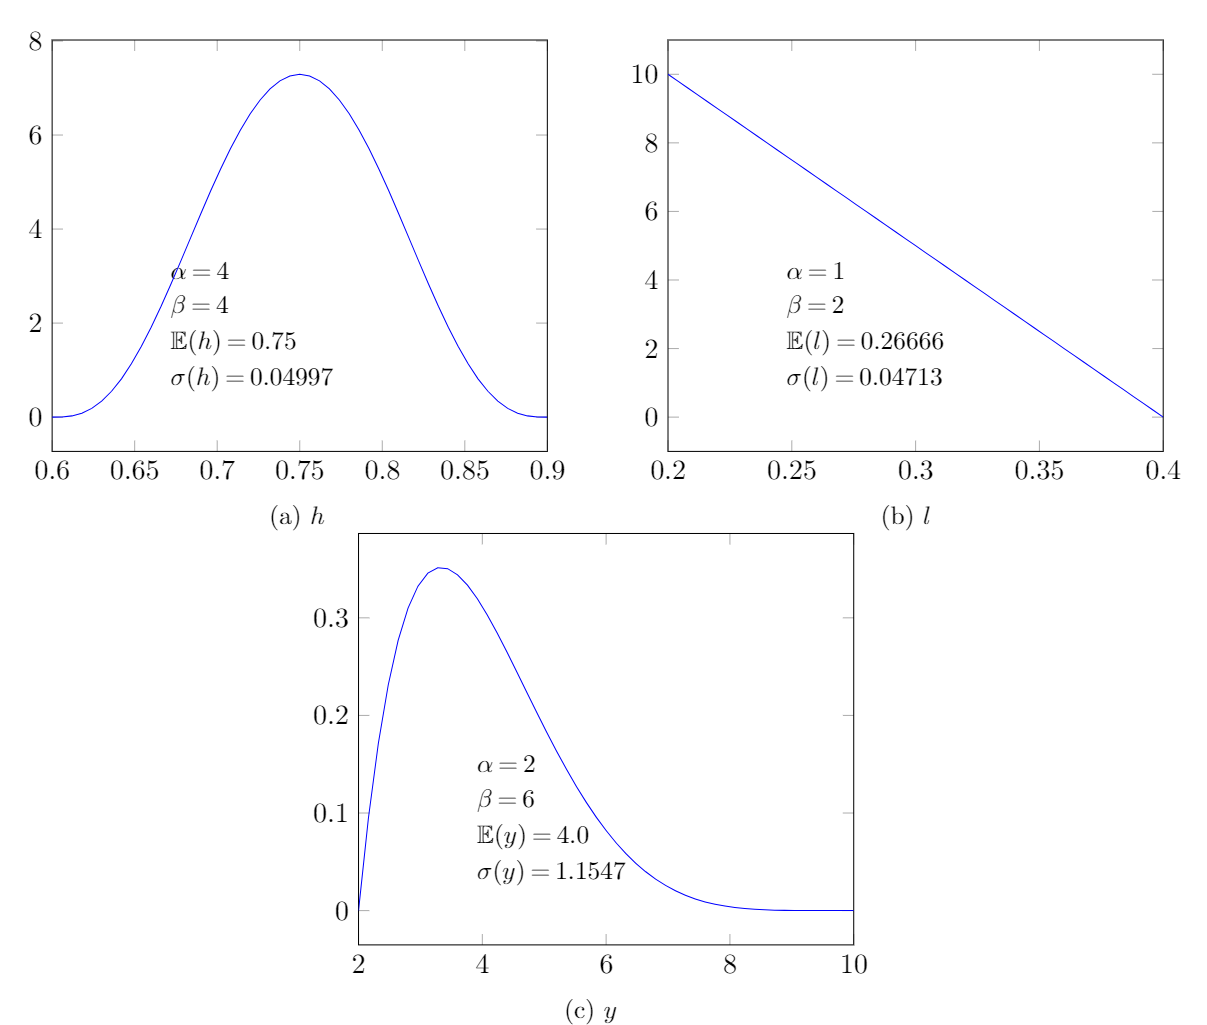
\includegraphics[scale=1]{figure1.png}
    \caption{Beta distributions for financial strength (a), local content (b), and ears of experience (c)}
    \label{figBeta}
\end{figure}

\begin{subequations} \label{eqBetaDist}
\begin{align}
	&\qquad \mathbb{E}(x_j) = \frac{\alpha_j x_j^{max}+\beta_j x_j^{min}}{\alpha_j+\beta_j}\label{eqBetaAvg}  \\
    &\qquad \sigma(x_j) = \frac{x_j^{max}-x_j^{min}}{\alpha_j\beta_j}\left(\frac{\alpha_j \beta_j}{\alpha_j+\beta_j+1}\right) ^{1/2}\label{eqBetaStd} 
\end{align}
\end{subequations}

We start by defining the beta distributions and targets for years of experience, financial strength, and local content plotted in figure \ref{figBeta}. The domain bounds on the horizontal axis represent the maximum and minimum values assigned to each distribution. 

The targeted minimum years of experience of the management team, $y^{0}$, is set to 5, and the optimal number of years of experience, $(y^{*})$, to 10. We define a symmetric beta distribution shown in figure (\ref{figBetay}) with the minimum set to 3 and the maximum set to $y^*$. The distribution is skewed towards a lower number of years with an expected value of 4 years and a standard deviation of 1.15. This reflects a concentration of bidders with an experience bellow the target, reflecting the relatively early stages of development of the Saudi electricity market.

The targeted financial strength $(h^{0})$, ratio of warranties to capital cost, is set to 0.75. This matches the gearing ratio reported by Bloomberg New Energy Finance (BNEF 2017) for the Al Mourjan plant, requiring generation companies to secure a relatively high level of financial instruments to win the contract. For the distribution we assume a minimum value of 0.6 and a maximum of 0.9, with a symmetric distribution.

The distribution of local content, shown in figure (\ref{figBetal}) is concentrated towards lower levels with minimum level of 20\%, a maximum level of 40\%. This reflects the fact that majority of equipment used in Saudi power generation projects needs to be sourced from international suppliers, given the lack of local manufacturing for the power industry. We assume a an expected value of 26.7\% and a standard deviation of 4.78\%. In the National Transformation Program (NTP 2017) the baseline percentage of local content in total expenditure by The Ministry of Energy Mineral and Mineral Resources is reported as 36\% with a benchmark of 50\%. Assuming the local content will be lower for power projects we select a targeted level $(l^{0})$ of 30\%. 

Other parameters related to years of experience, financial strength local content and the utilization factor are as follows. The slippage parameter increasing capital cost for each year of experience ($\tau$) is  set to  1\% of the total capital cost at the targeted level of local content. The slippage parameter for financial strength $(\mu)$  is set such that at the targeted level of financial strength and local content the capital cost increases by 10\%, (0.13\% for each percentage point of financial guarantees).  The initial utilization factor, defined as $\theta_0$, is set to 70\%. It is modified by the impact of local content $(\epsilon_l)$, set to -0.1\% for each percentage of local content used in the project,  plus the positive  impact of financial strength $(\epsilon_h)$, set to 0.05\% for each percent of financial warranties secured by the company. These values reflect how the generators decisions can impact their bid for project, but do not based on actual statistics.

The target energy and capacity prices are determined using reported investment and variable operating costs. The annualized capital cost of the Al Mourjan plant is calculated as 188 USD/KW assuming a 6\% discount rate for Saudi power sector investments (\citealp{Matar_et_al_2016}), for a 35 year lifetime. We set the benchmark annualized capital cost at 100\% international content to 73 USD/KW, using a capital cost of 1059 USD/KW as reported for a CCGT by \cite{Rioux_et_al_2017}, applying the same discount rate and lifetime. The capital cost under 100\% local content is set to 400 USD/KW, assuming that the reported capital cost for the Al Mourjan plant (188 USD/KW) corresponds to 30\%  local content, and includes the cost slippage for years of experience and financial strength.

We can see a significant difference between the benchmark (73 USD/KW) and reported capital cost of the Al Mourkan plant (188 USD/KW). One reasoning for this discrepancy could be that PPAs offer a very low price for energy with a small rent on production for producers. This can cause investors to markup the reported cost of capital to receive a higher capacity payment and return on investment from the capacity sold. 

 In the \textit{high capacity price} scenario the capacity price target is set to the annualized investment cost including the cost slippage terms (equation \ref{eqBuyerFixedCost}), at the targeted decisions $(l=l^{0}, y=y^{0}, h=h^{0})$,  adding a $7\%$ markup. The target energy price is set to the total of non-fuel and fuel variable operating costs, assuming a 50\% net efficiency for CCGT, also applying a $7\%$ markup.  We assume the government makes a compromise on fuel price reform targets, charging power producers 1.5 USD/mmbtu, $20\%$ higher than the current industrial rate (\citealp{Fattouh_2018}). We assume a non-fuel variable operating cost of 1.24 USD/MWH using values reported in \cite{Rioux_et_al_2017}, giving a total variable operating cost is 10.67 USD/KWh. We assume that under the target level of local content the operating costs increase by 5\% raising the overall operating cost and target energy price to 11.20 USD/MWh.

For the \textit{low capacity price} scenario we reduce the annualized capital cost (at 30\% local content) by 50\% to 94.0 USD/KW, offering a discount on the purchase of capital by private investors. This may require the government writing off a portion of SEC’s debt, still owned by the plant, but allows the buyer to commit to a higher energy price without significantly increasing the total cost of the contract.  Such a discount may be perceived as necessary by investors if the original cost is deemed to high compared to building a new plant. Under the the lower capital requirement fuel prices are increased to 3.95 USD/mmbtu as a hypothetical reform target, resulting in a higher variable operating cost, and energy price target, of  31.68USD/MWh (including the 5\% increase a the targeted level of local content).


The beta distributions of the energy and capacity price bids for all three scenarios are shown in figure (\ref{figBetaPrices}). The energy price bids range from the marginal cost $c$ at the targeted local content for each scenario (minimum) to a maximum of $1.05\%$ of $p^0$, while the capacity price bids range from the annualized capital cost in each scenario to a maximum of $1.05\%$ of $\delta^0$. We apply a symmetric bell shaped distribution for both prices. For the \textit{Higher volatility} scenario the beta distribution for the energy price is widened, increasing the standard deviation of the energy price from 0.32 to 0.44.

The results of the model, including the value of the rating function $(\phi)$, the probability of the bid being accepted $(\rho)$, the weights assigned by the buyer, cost of the contract, generator costs and total profits, are listed in table (\ref{tableResults}).
\begin{figure}
	\centering 
	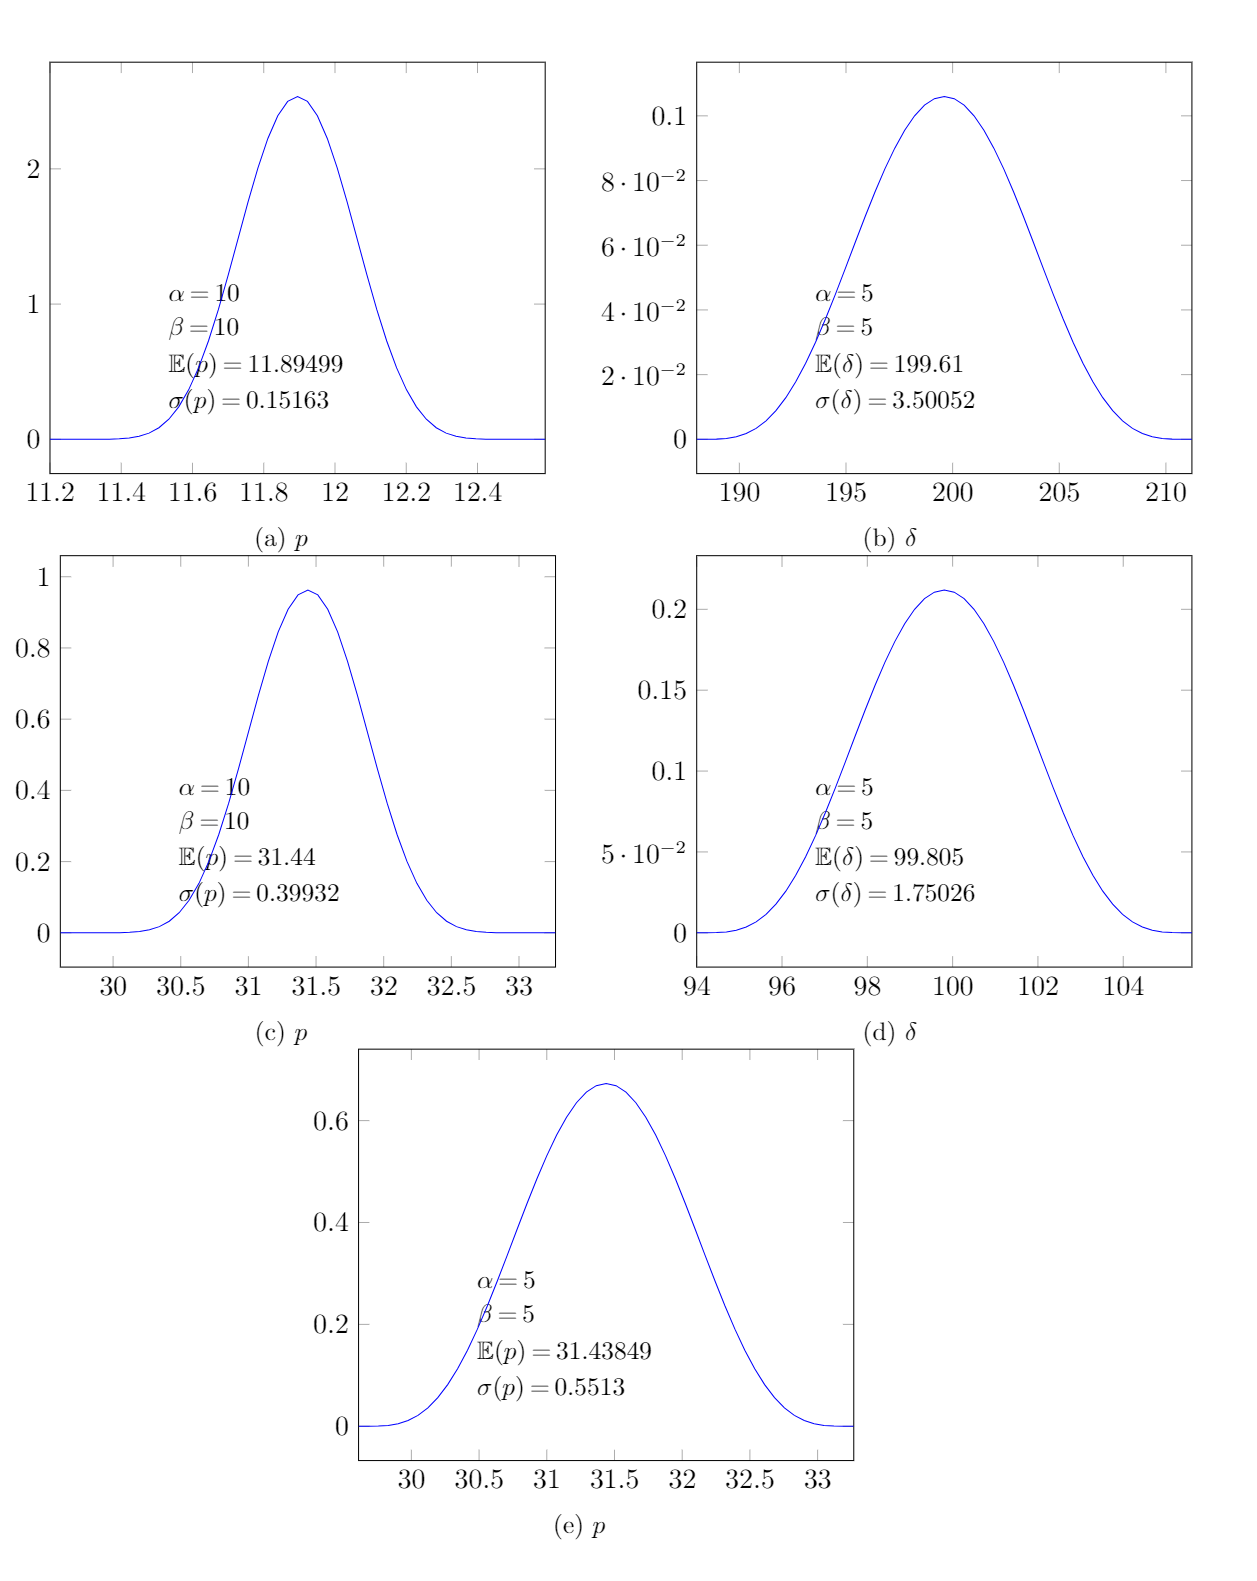
\includegraphics[scale=1]{figure2.png}
    \caption{Beta distributions of the energy price and capacity price for the $\textit{high capacity price}$ scenario, (a) and (b), and $\textit{low capacity price}$ scenario, (c) and (d), and beta distribution of the energy price under the $\textit{higher volatility} $ scenario (e)}
    \label{figBetaPrices}
\end{figure}


\begin{table}%[tableResults]
\caption {Rating, probability of bid acceptance, weights, contract cost, generator cost, and profit for each scenario} \label{tableResults}
\begin{tabular}{@{}llll@{}}
\toprule
Scenario                & \textit{High capacity price} & \textit{Low capacity price} & \textit{Lower price volatility} \\ \midrule
Rating, $\phi$          & 0.072                          & 0.175                         & 0.140                             \\
$\rho$                  & 0.518                          & 0.544                         & 0.535                             \\
$\omega_p$              & 0.101                          & 0.267                         & 0.298                             \\
$\omega_{\delta}$       & 0.396                          & 0.199                         & 0.191                             \\
$\omega_h$              & 0.066                          & 0.033                         & 0.032                             \\
$\omega_l$              & 0.437                          & 0.387                         & 0.370                             \\
$\omega_y$              &                                & 0.114                         & 0.109                             \\
PPA cost (bil \$)       & 1.039                          & 1.120                         & 1.120                             \\
Generator cost (bil \$) & 0.971                          & 1.049                         & 1.047                             \\
Profit (bil \$)         & 0.068                          & 0.072                         & 0.073                             \\ \bottomrule
\end{tabular}
\end{table}




\section{Conclusions}\label{Conclusions}


%%%%%%%%%%

\begin{thebibliography}{}
\bibitem[{Amorim et al. (2013)}]{Amorim_et_al_2013}	
Amorim, F., J. Vasconcelos, I. C. Abreu, P. P. Silva, V. Martins, 2013. “How Much Room for a Competitive Electricity Generation Market in Portugal.” \textit{Renewable and Sustainable Energy Reviews}, 18: 103-118.	
	
\bibitem[{Albadi (2017)}]{Albadi_2017}	
Albadi, 2017!!!!!!!!!!!!.	
	
	
\bibitem[{Asian Development Bank (2010)}]{Asian_Dev_Bank_2010}
Asian Development Bank. \textit{Guide on Bid Evaluation}. www.adb.org , October, 2010, pp. 195. 

\bibitem[{Capen et al. (1971)}]{Capen_et_al_1971}
Capen, E. E., R. V. Clapp, W. M. Campbell, 1971. “Competitive Bidding in High-Risk Situations." \textit{Journal of Petroleum Technology}, 23: 641-653.

\bibitem[{Cozzi (2012)}]{Cozzi_2012}
Cozzi, P. “Assessing Reverse Auctions as a Policy Tool for Renewable Energy Deployment,”  Energy, Climate, and Innovation Program, 7. The Center for International Environment \& Resource Policy, Tufts University, www.fletcher.tufts.edu/cierp, May, 2012, pp. 38.

\bibitem[{Chen (1989)}]{Chen_1989}
Chen, H., ”Competitive Bidding Strategy in the Construction Industry, Game Theoretic Approach,” Master of Science in Civil Engineering, Graduate School of the New Jersey Institute of Technology. May, 1989, pp. 92.

\bibitem[{Chua and Li (2000)}]{Chua_Li_2000}
Chua, D.K.H., D. Li, 2000. “Multiattribute Electronic Procurement Using Goal Programming.” \textit{Journal of Construction Engineering and Management}, 126 (5): 349-357.

\bibitem[{del Rio and Linares (2014)}]{delRio_Linares_2014}
del Rio, P., and P. Linares, 2014. “Back to the Future? Rethinking Auctions for Renewable Electricity Support.” \textit{Renewable and Sustainable Energy Reviews}, 35: 42-56.

\bibitem[{Eberhard (2007)}]{Eberhard_2007}
Eberhard, A., 2007. “From State to Market and Back Again: Egypt’s Experiment with Independent Power Projects.” \textit{Energy}, 32: 724-738.

\bibitem[{ECRA (2018)}]{ECRA_2018}
ECRA, 2018!!!!!!!!!!!!!!!!!!!!!!!!!!


\bibitem[{Ehrgott (2005)}]{Ehrgott_2005}
Ehrgott, M., “Multicriteria Optimization.” Second edition. Springer. 2005.

\bibitem[{Electric Power Supply Association (2004)}]{Electric_power_2004}
Electric Power Supply Association. Getting the Best Deal for Electricity Utility Customers. www.epsa.org. 2004, January, pp. 35.


\bibitem[{Falcom (2018)}]{Falcom_2018}
Falcom, 2018!!!!!!!!!!!!!!!!!!!!!!!!!!

\bibitem[{Fattouh (2018)}]{Fattouh_2018}
Fattouh, 2018!!!!!!!!!!!!!!!!!!!!!!!!!!!!

\bibitem[{Fiscal Balance Program (2018)}]{Fiscal_Balance_2018}	
Fiscal Balance Program, 2018  !!!!!!!!!!!!.	

\bibitem[{Gloabl Energy Observatory (2018)}[GEO] http://www.globalenergyobservatory.org/geoid/43689).]

\bibitem[{IRENA (2015)}]{IRENA_2015}
IRENA. “Renewable Energy Policies and Auctions,” www.irena.org, 2015, pp. 39.

\bibitem[{KEMA et al. (2013)}]{KEMA_et_al_2013}
KEMA, REKK and EIHP. “Development and Application of a Methodology to Identify Projects of Energy Community Interest.” KEMA Consulting GmbH.  September, 2013, pp. 92. 

\bibitem[{Kameshwaran et al. (2007)}]{Kameshwaran_et_al_2007}
Kameshwaran, S., Y. Narahari, C. H. Rosa, D. M. Kulkarni, J. D. Tew, 2007. “Multiattribute Electronic Procurement Using Goal Programming.” \textit{European Journal of Operational Research}, 179: 518-536.

\bibitem[{Kashi (2015)}]{Kashi_2015}
Kashi, B., 2015. “Risk Management and the Stated Investment Costs by Independent Power Producers.” \textit{Energy Economics}, 49: 660-668. 

\bibitem[{Kee (2001)}]{Kee_2001}
Kee, E. D., 2001. “Vesting Contracts: A Tool for Electricity Market Transition.” \textit{The Electricity Journal}, July: 11-22. 

\bibitem[{Liu et al. (2000)}]{Liu_et_al_2000}
Liu, S. L., K. K. Lai, and S. Y. Wang, 2000. “Multiple Criteria Models for Evaluation of Competitive Bids.” \textit{IMA Journal of Mathematics Applied in Business and Industry}, 11 (3): 151-160.


\bibitem[{Matar et al. (2016)}]{Matar_et_al_2016}
Matar et al. (2016)!!!!!!!!!!!!!!!!!!!!!!!!!!!!!!!


\bibitem[{Meland et al. (2011)}]{Meland_et_al_2011}
Meland, O. H., K. Robertsen, G. Hannas. “Selection Criteria and Tender Evaluation: The Equivalent Tender Price Model (ETPM).” In “Management and Innovation for a Sustainable Built Environment, The CIB conference MISBE2011, 20-23 June, 2011. 

\bibitem[{Merrimack Energy Group (2005)}]{Merrimack_2005}
Merrimack Energy Group. “Bid Evaluation and Selection Process For Wind-Generated Electricity For 1000 MW of Capacity Call for Tenders Process,” 2005, pp. 17.

\bibitem[{Nagayama (2007)}]{Nagayama_2007}
Nagayama, H., 2007. “Effects of Regulatory Reforms in the Electricity Supply Industry on Electricity Prices in Developing Countries.” \textit{Energy Policy}, 35: 3440-3462. 

\bibitem[{NREL (2009)}]{NREL_2009}
National Renewable Energy Laboratory (NREL). “Power Purchase Agreement Checklist for State and Local Governments.” Energy Analysis, 2009, pp. 11. 

\bibitem[{Newbery (2016)}]{Newbery_2016}
Newbery, D., 2016. “Tales of two islands – Lessons for EU Energy Policy From Electricity Market Reforms in Britain and Ireland.” \textit{Energy Policy}, 105(C): 597-607. 

\bibitem[{Phadke (2009)}]{Phadke_2009}
Phadke, A., 2009. “How many Enrons? Mark-ups in the Stated Capital Cost of Independent Power Producers’ (IPPs’) Power Projects in Developing Countries.” \textit{Energy}, 34: 1917-1924.

\bibitem[{Phillips (2005)}]{Phillips_2005}
Phillips, R. L., \textit{Pricing and Revenue Optimization}. Stanford University Press, 2005. 


\bibitem[{RCREEE (2012)}]{RCREEE_2012}
Regional Center for Renewable Energy and Energy Efficiency (RCREEE). “USER’S GUIDE for The Power Purchase Agreement (PPA) Model For Electricity Generated From Renewable Energy Facilities.” www.rcreee.org, 2012, pp. 17.


\bibitem[{Rego and Parente (2013)}]{Rego_Parente_2013}
Rego, E. E., and V. Parente, 2013. “Brazilian Experience in Electricity Auctions: Comparing Outcomes From New and Old Energy Auctions as Well as the Application of the Hybrid Anglo-Dutch design,” Energy Policy, 55: 511-520. 

\bibitem[{Rioux et al. (2017)}]{Rioux_et_al_2017}
Rioux et al. (2017)!!!!!!!!!!!!!!!!!!!!!!!!!!!!!!!


\bibitem[{Santiago and Roxas (2010)}]{Santiago_Roxas_2010}
Santiago, A., and F. Roxas, 2010. “Understanding Electricity Market Reforms and the Case of Philippine Deregulation.” \textit{The Electricity Journal}, 23 (2): 48-57. 

\bibitem[{Shih (2007)}]{Shih_2007}
Shih, H.-C., 2007. “Evaluating the Prospective Effects of Alternative Regulatory Policies on the Investment Behaviour and Environmental Performance of a Newly Liberalised Electricity Industry in Taiwan.” \textit{Socio-Economic Planning Sciences}, 41: 320-335. 

\bibitem[{Shrimali et al. (2016)}]{Shrimali_2016}
Shrimali, G., C. Konda, A. A. Farooquee. 2016. “Designing Renewable Energy Auctions for India: Managing Risks to Maximize Deployment and Cost-Effectiveness.” \textit{Renewable Energy}, 97: 656-670. 

\bibitem[{Taha (2007)}]{Taha_2007}
Taha, H. A., “Operations Research, An Introduction.” Eighth edition. Pearson Prentice Hall. 2007.


\end{thebibliography}


%% Here starts the e-companion (EC)
%%%%%%%%%%%%%%%%%%%%%%%%%%%%%%%%%%%%%%%%%%%%%%%%%%%%%%%%%%
%\ECSwitch

%\ECDisclaimer
%%%%%%%%%%%%%%%%%%%%%%%%%%%%%%%%%%%%%%%%%%%%%%%%%%%%%%%%%%

%%% Main head for the e-companion
%\ECHead{Online Appendix}
%\begin{APPENDICES}
%A general heading for the whole e-companion should be provided here as in the example above this paragraph.


% Appendix here
% Options are (1) APPENDIX (with or without general title) or
%             (2) APPENDICES (if it has more than one unrelated sections)
% Outcomment the appropriate case if necessary
%
%\newpage
% \begin{APPENDICES}{}
% 
%
%   or
%
% \begin{APPENDICES}
% \section{<Title of Section A>}
% \section{<Title of Section B>}
% etc
% \end{APPENDICES}

%\begin{APPENDICES}
%\section{Derivation of the spot market outcomes (\ref{prop_S})-(\ref{prop_qS})}\label{Appendix_prop_lin_equi}

%\section{Concavity characterization and first order optimal conditions for problems (\ref{eq3.9}) and (\ref{eq3.10})}\label{Appendix_C}


%\end{APPENDICES}


% Acknowledgments here
%\ACKNOWLEDGMENT{The authors gratefully acknowledge the existence of
%the Journal of Irreproducible Results and the support of the Society
%for the Preservation of Inane Research.}


% References here (outcomment the appropriate case)

% CASE 1: BiBTeX used to constantly update the references
%   (while the paper is being written).
%\bibliographystyle{ormsv080} % outcomment this and next line in Case 1
%\bibliography{<your bib file(s)>} % if more than one, comma separated

% CASE 2: BiBTeX used to generate mypaper.bbl (to be further fine tuned)
%\input{mypaper.bbl} % outcomment this line in Case 2

%If you don't use BiBTex, you can manually itemize references as shown below.


%%%%%%%%%%%%%%%%%
\end{document}
%%%%%%%%%%%%%%%%%





